\documentclass[11pt,a4paper]{article}
\setlength{\headheight}{14pt}
\usepackage[margin=1in]{geometry}
\usepackage{amsmath}
\usepackage{amssymb}
\usepackage{titlesec}
\usepackage{enumitem}
\usepackage{xcolor}
\usepackage[most]{tcolorbox}
\usepackage{fancyhdr}
\usepackage{listings}
\usepackage{hyperref}
\usepackage{graphicx}
\usepackage{tikz}
\usetikzlibrary{shapes.geometric, arrows, positioning}

\usepackage{amssymb}
\usepackage{newunicodechar}

\newunicodechar{✅}{\checkmark}
\newunicodechar{❌}{\ding{55}} % requires pifont
\newunicodechar{≠}{\neq}

\usepackage{pifont}

\DeclareUnicodeCharacter{2502}{|}
\DeclareUnicodeCharacter{251C}{+}
\DeclareUnicodeCharacter{2500}{-}
\DeclareUnicodeCharacter{2514}{+}

% Header and Footer
\pagestyle{fancy}
\fancyhf{}
\rhead{MLflow Complete Guide}
\lhead{Experiment Tracking \& Model Registry}
\cfoot{\thepage}

% Title formatting
\titleformat{\section}{\Large\bfseries\color{blue!70!black}}{\thesection}{1em}{}[\titlerule]
\titleformat{\subsection}{\large\bfseries\color{blue!50!black}}{\thesubsection}{1em}{}
\titleformat{\subsubsection}{\normalsize\bfseries\color{blue!40!black}}{\thesubsubsection}{1em}{}

% Code styling
\definecolor{codebg}{gray}{0.95}
\definecolor{codegreen}{rgb}{0,0.6,0}
\definecolor{codegray}{rgb}{0.5,0.5,0.5}
\definecolor{codepurple}{rgb}{0.58,0,0.82}

\lstdefinestyle{pythonstyle}{
    language=Python,
    backgroundcolor=\color{codebg},
    commentstyle=\color{codegreen},
    keywordstyle=\color{blue},
    numberstyle=\tiny\color{codegray},
    stringstyle=\color{codepurple},
    basicstyle=\ttfamily\small,
    breaklines=true,
    captionpos=b,
    keepspaces=true,
    numbers=left,
    numbersep=5pt,
    showspaces=false,
    showstringspaces=false,
    showtabs=false,
    tabsize=4,
    frame=single,
    xleftmargin=2em,
    framexleftmargin=1.5em
}

\lstdefinestyle{bashstyle}{
    language=bash,
    backgroundcolor=\color{codebg},
    basicstyle=\ttfamily\small,
    breaklines=true,
    frame=single,
    xleftmargin=2em,
    framexleftmargin=1.5em
}

\lstset{style=pythonstyle}

% Command box
\newtcolorbox{cmdbox}{
    colback=codebg,
    colframe=black!50,
    boxrule=0.5pt,
    left=2mm,
    right=2mm,
    top=1mm,
    bottom=1mm,
    breakable,
    enhanced jigsaw
}

% Example box
\newtcolorbox{examplebox}[1]{
    colback=green!5!white,
    colframe=green!75!black,
    title=#1,
    fonttitle=\bfseries,
    breakable,
    enhanced jigsaw
}

% Note box
\newtcolorbox{notebox}{
    colback=yellow!10!white,
    colframe=orange!75!black,
    title=Important Note,
    fonttitle=\bfseries,
    breakable,
    enhanced jigsaw
}

% Warning box
\newtcolorbox{warningbox}{
    colback=red!5!white,
    colframe=red!75!black,
    title=Warning,
    fonttitle=\bfseries,
    breakable,
    enhanced jigsaw
}

% Info box
\newtcolorbox{infobox}[1]{
    colback=blue!5!white,
    colframe=blue!75!black,
    title=#1,
    fonttitle=\bfseries,
    breakable,
    enhanced jigsaw
}

\begin{document}

% Title Page
\begin{titlepage}
    \centering
    \vspace*{2cm}
    {\Huge\bfseries MLflow\\[0.5cm] Complete Guide\par}
    \vspace{1cm}
    {\Large Experiment Tracking \& Model Registry\par}
    \vspace{2cm}
    {\large A Comprehensive Guide to MLflow for Machine Learning\\
    Experiment Tracking, Model Registry, and Production Deployment\par}
    \vspace{3cm}
    {\Large\bfseries Sujil S\par}
    \vspace{0.5cm}
    {\large\texttt{sujil9480@gmail.com}\par}
    \vfill
    {\large \today\par}
\end{titlepage}

\tableofcontents
\newpage

% ========================
% SECTION 1: INTRODUCTION
% ========================
\section{Introduction to MLflow}

\subsection{What is MLflow?}

\textbf{MLflow} is an open-source platform designed to manage the complete machine learning lifecycle. It provides tools for experiment tracking, model versioning, deployment, and collaboration.

\begin{infobox}{Core MLflow Components}
\begin{enumerate}[leftmargin=*]
    \item \textbf{MLflow Tracking}: Log and query experiments (parameters, metrics, artifacts)
    \item \textbf{MLflow Projects}: Package ML code in reusable, reproducible format
    \item \textbf{MLflow Models}: Manage and deploy models from various ML libraries
    \item \textbf{MLflow Model Registry}: Centralized model store for managing model lifecycle
\end{enumerate}
\end{infobox}

\subsection{The Experimentation Challenge}

In machine learning projects, multiple experiments are conducted at each pipeline stage:

\begin{itemize}[leftmargin=*]
    \item \textbf{Pre-Processing}: E1, E2, E3, ...
    \begin{itemize}
        \item E1: Handling outliers using IQR
        \item E2: Handling outliers using Isolation Forest
        \item E3: Different scaling techniques
    \end{itemize}
    
    \item \textbf{Feature Engineering}: E1, E2, E3, ...
    \begin{itemize}
        \item Different feature selection methods
        \item Various feature transformation techniques
        \item Multiple feature combinations
    \end{itemize}
    
    \item \textbf{Model Selection}: E1, E2, E3, ...
    \begin{itemize}
        \item Random Forest vs XGBoost vs Neural Networks
        \item Different algorithm families
    \end{itemize}
    
    \item \textbf{Hyperparameter Tuning}: E1, E2, E3, ...
    \begin{itemize}
        \item Grid search combinations
        \item Random search trials
        \item Bayesian optimization iterations
    \end{itemize}
\end{itemize}

\begin{notebox}
After conducting numerous experiments across all stages, we need to identify the combination that provides the best results. Industry-grade tools like \textbf{DVC} and \textbf{MLflow} are essential for managing this complexity.
\end{notebox}

\newpage

% ========================
% SECTION 2: DVC VS MLFLOW
% ========================
\section{DVC vs MLflow Comparison}

\subsection{Evolution and Purpose}

\subsubsection{DVC (Data Version Control)}

\begin{itemize}[leftmargin=*]
    \item \textbf{Initial Purpose}: Data versioning only
    \item \textbf{Evolution}: Added experiment tracking after gaining popularity
    \item \textbf{Inspiration}: Experiment tracking inspired by MLflow
    \item \textbf{Maturity}: Newer to experiment tracking compared to MLflow
\end{itemize}

\subsubsection{MLflow}

\begin{itemize}[leftmargin=*]
    \item \textbf{Purpose-Built}: Designed from the ground up for ML lifecycle management
    \item \textbf{Maturity}: More mature and feature-complete for experiment tracking
    \item \textbf{Flexibility}: Can be used independently without Git
\end{itemize}

\subsection{Key Differences}

\begin{center}
\begin{tabular}{|p{0.45\textwidth}|p{0.45\textwidth}|}
\hline
\textbf{DVC} & \textbf{MLflow} \\
\hline
Must be used with Git & Can be used without Git \\
\hline
UI is basic and less intuitive & Rich, user-friendly web UI \\
\hline
Experiment history is local only & Allows team-wide collaboration \\
\hline
Primarily for data versioning & Comprehensive ML lifecycle management \\
\hline
No centralized experiment tracking & Centralized tracking server available \\
\hline
Limited visualization capabilities & Advanced visualization and comparison tools \\
\hline
\end{tabular}
\end{center}

\subsection{Why MLflow is Preferred}

Due to the following advantages, \textbf{MLflow is given higher priority} in industry for experiment tracking:

\begin{enumerate}[leftmargin=*]
    \item \textbf{Superior UI/UX}: Intuitive web interface for experiment comparison
    \item \textbf{Team Collaboration}: Centralized server allows entire team to view and compare experiments
    \item \textbf{Independence}: Works standalone without requiring Git
    \item \textbf{Maturity}: More stable and feature-complete for experiment tracking
    \item \textbf{Comprehensive Features}: Covers entire ML lifecycle, not just data versioning
\end{enumerate}

\subsection{MLflow Capabilities Beyond Experiment Tracking}

\begin{itemize}[leftmargin=*]
    \item \textbf{Visualization}: Interactive plots and metrics comparison
    \item \textbf{Generative AI}: Support for LLM tracking and evaluation
    \item \textbf{Evaluation}: Built-in model evaluation frameworks
    \item \textbf{Model Registry}: Complete model lifecycle management
    \item \textbf{Serving}: Model deployment and serving capabilities
    \item \textbf{Models}: Standardized model format for various frameworks
\end{itemize}

\newpage

% ========================
% SECTION 3: INITIAL SETUP
% ========================
\section{Getting Started with MLflow}

\subsection{Installation and Setup}

\subsubsection{Step 1: Create Repository}

\begin{cmdbox}
\begin{verbatim}
# Create a new repository on GitHub
# Clone it locally
git clone https://github.com/username/mlflow-project.git
cd mlflow-project
\end{verbatim}
\end{cmdbox}

\subsubsection{Step 2: Install MLflow}

\begin{cmdbox}
\begin{verbatim}
# Install MLflow
pip install mlflow

# Verify installation
mlflow --version
\end{verbatim}
\end{cmdbox}

\subsubsection{Step 3: Launch MLflow UI}

\begin{cmdbox}
\begin{verbatim}
# Start MLflow UI
mlflow ui
\end{verbatim}
\end{cmdbox}

\textbf{What happens}:
\begin{itemize}[leftmargin=*]
    \item MLflow UI starts at \texttt{http://127.0.0.1:5000}
    \item Creates \texttt{mlflow.db} file (SQLite database for metadata)
    \item Ready to receive experiment data
\end{itemize}

\subsubsection{Step 4: Create Project Structure}

\begin{cmdbox}
\begin{verbatim}
# Create source folder
mkdir src
cd src
\end{verbatim}
\end{cmdbox}

\textbf{Project structure}:
\begin{verbatim}
mlflow-project/
├── src/
│   ├── main_1.py
│   ├── main_2.py
│   └── ...
├── mlflow.db
├── mlartifacts/
└── mlruns/
\end{verbatim}

\subsection{Understanding MLflow Storage}

\begin{infobox}{Storage Locations}
\textbf{Where artifacts are stored depends on setup}:

\begin{center}
\begin{tabular}{|l|l|}
\hline
\textbf{Setup} & \textbf{Artifact Folder} \\
\hline
File-based tracking & mlruns/ \\
\hline
MLflow server & mlartifacts/ \\
\hline
Dagshub (remote) & Remote (no local folder) \\
\hline
\end{tabular}
\end{center}

\textbf{Key Point}: Artifacts are stored differently based on the artifact store configuration. Local tracking uses \texttt{mlruns/}, while server-based tracking uses \texttt{mlartifacts/}.
\end{infobox}

\newpage

% ========================
% SECTION 4: BASIC MLFLOW USAGE
% ========================
\section{Basic MLflow Experiment Tracking}

\subsection{First MLflow Script}

\begin{examplebox}{main\_1.py - Basic Experiment}
\begin{lstlisting}[language=Python]
import mlflow
import mlflow.sklearn
from sklearn.datasets import load_wine
from sklearn.ensemble import RandomForestClassifier
from sklearn.model_selection import train_test_split
from sklearn.metrics import accuracy_score, confusion_matrix
import matplotlib.pyplot as plt
import seaborn as sns

mlflow.set_tracking_uri("http://127.0.0.1:5000")

# Load Wine dataset
wine = load_wine()
X = wine.data
y = wine.target

# Train test split
X_train, X_test, y_train, y_test = train_test_split(
    X, y, test_size=0.10, random_state=42
)

# Define the params for RF model
max_depth = 10
n_estimators = 5

with mlflow.start_run():
    rf = RandomForestClassifier(
        max_depth=max_depth, 
        n_estimators=n_estimators, 
        random_state=42
    )
    rf.fit(X_train, y_train)

    y_pred = rf.predict(X_test)
    accuracy = accuracy_score(y_test, y_pred)

    mlflow.log_metric('accuracy', accuracy)
    mlflow.log_param('max_depth', max_depth)
    mlflow.log_param('n_estimators', n_estimators)

    # Creating a confusion matrix plot
    cm = confusion_matrix(y_test, y_pred)
    plt.figure(figsize=(6,6))
    sns.heatmap(cm, annot=True, fmt='d', cmap='Blues', 
                xticklabels=wine.target_names, 
                yticklabels=wine.target_names)
    plt.ylabel('Actual')
    plt.xlabel('Predicted')
    plt.title('Confusion Matrix')

    # save plot
    plt.savefig("Confusion-matrix.png")

    # log artifacts using mlflow
    mlflow.log_artifact("Confusion-matrix.png")
    mlflow.log_artifact(__file__) # for saving the current script

    # tags
    mlflow.set_tags({
        "Author": 'Sujil S', 
        "Project": "Wine Classification"
    })

    # Log the model
    mlflow.sklearn.log_model(rf, "Random-Forest-Model")

    print(accuracy)
\end{lstlisting}
\end{examplebox}

\subsection{Running the Script}

\begin{cmdbox}
\begin{verbatim}
# Run the script
python src/main_1.py
\end{verbatim}
\end{cmdbox}

\textbf{What happens}:
\begin{enumerate}[leftmargin=*]
    \item Creates \texttt{mlartifacts/} folder
    \item Stores plot, model, and Python script
    \item Run is stored in default experiment (ID: 0)
    \item Unique Run ID is generated
    \item All data visible in MLflow UI at \texttt{http://127.0.0.1:5000}
\end{enumerate}

\newpage

% ========================
% SECTION 5: WHAT CAN BE LOGGED
% ========================
\section{What Can Be Logged in MLflow}

\subsection{Complete Logging Capabilities}

\subsubsection{1. Metrics}

\textbf{Numeric values tracked over time}:

\begin{itemize}[leftmargin=*]
    \item \textbf{Accuracy}: Model accuracy across runs
    \item \textbf{Loss}: Training and validation loss during training
    \item \textbf{Precision, Recall, F1-Score}: Classification metrics
    \item \textbf{AUC (Area Under Curve)}: Classification performance
    \item \textbf{Custom Metrics}: Any numeric value (RMSE, MAE, etc.)
\end{itemize}

\begin{examplebox}{Logging Metrics}
\begin{lstlisting}[language=Python]
mlflow.log_metric('accuracy', 0.95)
mlflow.log_metric('precision', 0.92)
mlflow.log_metric('recall', 0.94)
mlflow.log_metric('f1_score', 0.93)
mlflow.log_metric('auc', 0.96)
\end{lstlisting}
\end{examplebox}

\subsubsection{2. Parameters}

\textbf{Configuration values for the run}:

\begin{itemize}[leftmargin=*]
    \item \textbf{Model Hyperparameters}: Learning rate, number of trees, max depth
    \item \textbf{Data Processing Parameters}: Train-test split ratio, preprocessing steps
    \item \textbf{Feature Engineering}: Feature selection criteria, transformation parameters
\end{itemize}

\begin{examplebox}{Logging Parameters}
\begin{lstlisting}[language=Python]
mlflow.log_param('learning_rate', 0.01)
mlflow.log_param('n_estimators', 100)
mlflow.log_param('max_depth', 10)
mlflow.log_param('test_size', 0.2)
\end{lstlisting}
\end{examplebox}

\subsubsection{3. Artifacts}

\textbf{Files and objects associated with the run}:

\begin{itemize}[leftmargin=*]
    \item \textbf{Trained Models}: Serialized model files
    \item \textbf{Model Summaries}: Architecture details, model info
    \item \textbf{Confusion Matrices}: Classification performance visualizations
    \item \textbf{ROC Curves}: Receiver Operating Characteristic curves
    \item \textbf{Plots}: Loss curves, feature importance plots
    \item \textbf{Input Data}: Training and testing datasets
    \item \textbf{Scripts \& Notebooks}: Code files, Jupyter notebooks
    \item \textbf{Environment Files}: requirements.txt, conda.yaml
\end{itemize}

\begin{examplebox}{Logging Artifacts}
\begin{lstlisting}[language=Python]
# Log individual files
mlflow.log_artifact("confusion_matrix.png")
mlflow.log_artifact("model_summary.txt")
mlflow.log_artifact(__file__)  # Current script

# Log entire directory
mlflow.log_artifacts("plots/")
\end{lstlisting}
\end{examplebox}

\subsubsection{4. Models}

\textbf{Serialized models in various formats}:

\begin{itemize}[leftmargin=*]
    \item \textbf{Pickled Models}: Python pickle format
    \item \textbf{ONNX Models}: Cross-platform ONNX format
    \item \textbf{Custom Models}: Using MLflow's model interface
\end{itemize}

\begin{examplebox}{Logging Models}
\begin{lstlisting}[language=Python]
# Log scikit-learn model
mlflow.sklearn.log_model(model, "model")

# Log TensorFlow model
mlflow.tensorflow.log_model(model, "tf-model")

# Log PyTorch model
mlflow.pytorch.log_model(model, "pytorch-model")
\end{lstlisting}
\end{examplebox}

\subsubsection{5. Tags}

\textbf{Metadata for organizing and filtering runs}:

\begin{itemize}[leftmargin=*]
    \item \textbf{Run Tags}: Author name, experiment description, model type
    \item \textbf{Environment Tags}: GPU usage, cloud provider
\end{itemize}

\begin{examplebox}{Setting Tags}
\begin{lstlisting}[language=Python]
mlflow.set_tags({
    "Author": "Sujil S",
    "Project": "Wine Classification",
    "Model": "RandomForest",
    "Environment": "GPU"
})
\end{lstlisting}
\end{examplebox}

\subsubsection{6. Source Code}

\textbf{Code versioning and tracking}:

\begin{itemize}[leftmargin=*]
    \item \textbf{Scripts}: Python files, notebooks
    \item \textbf{Git Commit}: Git commit hash
    \item \textbf{Dependencies}: Library versions
\end{itemize}

\begin{examplebox}{Logging Source Information}
\begin{lstlisting}[language=Python]
# Log current script
mlflow.log_artifact(__file__)

# Git information is automatically captured
# Dependencies can be logged with conda or requirements
\end{lstlisting}
\end{examplebox}

\subsubsection{7. Logging Inputs and Outputs}

\textbf{Data tracking}:

\begin{itemize}[leftmargin=*]
    \item \textbf{Training Data}: Input datasets
    \item \textbf{Test Data}: Validation/test datasets
    \item \textbf{Inference Outputs}: Model predictions
\end{itemize}

\begin{examplebox}{Logging Datasets}
\begin{lstlisting}[language=Python]
import mlflow.data

# Log training data
train_df = mlflow.data.from_pandas(train_dataframe)
mlflow.log_input(train_df, "training")

# Log test data
test_df = mlflow.data.from_pandas(test_dataframe)
mlflow.log_input(test_df, "testing")
\end{lstlisting}
\end{examplebox}

\subsubsection{8. Custom Logging}

\textbf{Flexible logging for any object}:

\begin{itemize}[leftmargin=*]
    \item \textbf{Custom Objects}: Any Python object
    \item \textbf{Custom Functions}: Track custom processing functions
\end{itemize}

\subsubsection{9. Model Registry}

\textbf{Model lifecycle management}:

\begin{itemize}[leftmargin=*]
    \item \textbf{Model Versioning}: Track different versions
    \item \textbf{Model Deployment}: Manage deployment status
    \item \textbf{Lifecycle Stages}: Staging, Production, Archived
\end{itemize}

\subsubsection{10. Run and Experiment Details}

\textbf{Metadata automatically captured}:

\begin{itemize}[leftmargin=*]
    \item \textbf{Run ID}: Unique identifier for each run
    \item \textbf{Experiment Name}: Logical grouping
    \item \textbf{Timestamps}: Start and end times
\end{itemize}

\newpage

% ========================
% SECTION 6: TRACKING URI
% ========================
\section{Understanding Tracking URI}

\subsection{The Tracking URI Problem}

\begin{warningbox}
\textbf{Common Error}: When \texttt{mlflow.set\_tracking\_uri()} is not specified, artifact logging may fail with:

\begin{verbatim}
mlflow.exceptions.MlflowException: When an mlflow-artifacts 
URI was supplied, the tracking URI must be a valid http or 
https URI, but it was currently set to sqlite:/mlflow.db.
\end{verbatim}
\end{warningbox}

\subsection{Understanding the Issue}

\begin{examplebox}{test.py - Checking Tracking URI}
\begin{lstlisting}[language=Python]
import mlflow

print("Printing tracking URI scheme below")
print(mlflow.get_tracking_uri())
print("\n")

mlflow.set_tracking_uri("http://127.0.0.1:5000")
print("Printing new tracking URI scheme below")
print(mlflow.get_tracking_uri())
print("\n")
\end{lstlisting}
\end{examplebox}

\textbf{Output}:
\begin{cmdbox}
\begin{verbatim}
Printing tracking URI scheme below
sqlite:///mlflow.db

Printing new tracking URI scheme below
http://127.0.0.1:5000
\end{verbatim}
\end{cmdbox}

\subsection{Why the Error Occurs}

\begin{infobox}{Root Cause}
The error occurs because:

\begin{enumerate}[leftmargin=*]
    \item By default, MLflow uses \textbf{SQLite backend}: \texttt{sqlite:///mlflow.db}
    \item Some experiments have artifact location set to \textbf{mlflow-artifacts://}
    \item The \texttt{mlflow-artifacts://} scheme requires an \textbf{HTTP/HTTPS server}
    \item SQLite backend is not in HTTP format
    \item When logging artifacts, MLflow cannot resolve the URI
\end{enumerate}
\end{infobox}

\subsection{The Solution}

\textbf{Always set tracking URI to HTTP format}:

\begin{lstlisting}[language=Python]
import mlflow

# Set tracking URI to MLflow server
mlflow.set_tracking_uri("http://127.0.0.1:5000")

# Now artifact logging will work
with mlflow.start_run():
    mlflow.log_artifact("plot.png")  # Works!
\end{lstlisting}

\subsection{MLflow Data Storage}

\begin{notebox}
All information for MLflow UI is obtained from two sources:

\begin{enumerate}[leftmargin=*]
    \item \textbf{mlflow.db}: Metadata (runs, experiments, parameters, metrics)
    \item \textbf{mlartifacts/} or \textbf{mlruns/}: Actual artifacts (models, plots, files)
\end{enumerate}
\end{notebox}

\newpage

% ========================
% SECTION 7: DELETING RUNS
% ========================
\section{Managing Runs and Experiments}

\subsection{Deleting Runs}

\subsubsection{UI Deletion (Soft Delete)}

\textbf{Method}: Using MLflow UI

\begin{enumerate}[leftmargin=*]
    \item Navigate to the run in UI
    \item Click delete button
    \item Run disappears from UI
\end{enumerate}

\begin{warningbox}
\textbf{Important}: UI deletion is a \textbf{soft delete}:

\begin{itemize}[leftmargin=*]
    \item Run is NOT removed from \texttt{mlflow.db}
    \item Run still exists in database with \texttt{lifecycle\_stage = deleted}
    \item It is hidden from UI but remains in the database
    \item Can be recovered if needed
\end{itemize}
\end{warningbox}

\subsubsection{Programmatic Deletion (Hard Delete)}

\textbf{Method}: Delete directly from database

\begin{examplebox}{Delete\_Runs.py}
\begin{lstlisting}[language=Python]
import mlflow

# Delete run by ID
mlflow.delete_run("Run_ID")
\end{lstlisting}
\end{examplebox}

\begin{cmdbox}
\begin{verbatim}
# Run deletion script
python Delete_Runs.py
\end{verbatim}
\end{cmdbox}

\textbf{Effect}: Deleting here removes the run from both UI and database.

\subsection{Creating Custom Experiments}

Instead of using the default experiment (ID: 0), create custom experiments for better organization.

\subsubsection{Method 1: Using MLflow UI}

\begin{enumerate}[leftmargin=*]
    \item Open MLflow UI
    \item Click "Create Experiment"
    \item Enter experiment name
    \item Obtain Experiment ID
    \item Use in code: \texttt{mlflow.start\_run(experiment\_id=<id>)}
\end{enumerate}

\begin{examplebox}{main\_2.py - Using Experiment ID}
\begin{lstlisting}[language=Python]
import mlflow
import mlflow.sklearn
from sklearn.datasets import load_wine
from sklearn.ensemble import RandomForestClassifier
from sklearn.model_selection import train_test_split
from sklearn.metrics import accuracy_score, confusion_matrix
import matplotlib.pyplot as plt
import seaborn as sns

# Load Wine dataset
wine = load_wine()
X = wine.data
y = wine.target

# Train test split
X_train, X_test, y_train, y_test = train_test_split(
    X, y, test_size=0.10, random_state=42
)

# Define the params for RF model
max_depth = 10
n_estimators = 15

# Use specific experiment by ID
with mlflow.start_run(experiment_id=1):
    rf = RandomForestClassifier(
        max_depth=max_depth, 
        n_estimators=n_estimators, 
        random_state=42
    )
    rf.fit(X_train, y_train)

    y_pred = rf.predict(X_test)
    accuracy = accuracy_score(y_test, y_pred)

    mlflow.log_metric('accuracy', accuracy)
    mlflow.log_param('max_depth', max_depth)
    mlflow.log_param('n_estimators', n_estimators)

    # Creating a confusion matrix plot
    cm = confusion_matrix(y_test, y_pred)
    plt.figure(figsize=(6,6))
    sns.heatmap(cm, annot=True, fmt='d', cmap='Blues', 
                xticklabels=wine.target_names, 
                yticklabels=wine.target_names)
    plt.ylabel('Actual')
    plt.xlabel('Predicted')
    plt.title('Confusion Matrix')

    # save plot
    plt.savefig("Confusion-matrix.png")

    # log artifacts using mlflow
    mlflow.log_artifact("Confusion-matrix.png")
    mlflow.log_artifact(__file__)

    # tags
    mlflow.set_tags({
        "Author": 'Sujil S', 
        "Project": "Wine Classification"
    })

    # Log the model
    mlflow.sklearn.log_model(rf, "Random-Forest-Model")

    print(accuracy)
\end{lstlisting}
\end{examplebox}

\subsubsection{Method 2: Programmatic Creation}

\textbf{Better approach}: Create experiment in code

\begin{examplebox}{main\_3.py - Using set\_experiment()}
\begin{lstlisting}[language=Python]
import mlflow
import mlflow.sklearn
from sklearn.datasets import load_wine
from sklearn.ensemble import RandomForestClassifier
from sklearn.model_selection import train_test_split
from sklearn.metrics import accuracy_score, confusion_matrix
import matplotlib.pyplot as plt
import seaborn as sns

mlflow.set_tracking_uri("http://127.0.0.1:5000")

# Load Wine dataset
wine = load_wine()
X = wine.data
y = wine.target

# Train test split
X_train, X_test, y_train, y_test = train_test_split(
    X, y, test_size=0.10, random_state=42
)

# Define the params for RF model
max_depth = 10
n_estimators = 15

# Set experiment by name (creates if doesn't exist)
mlflow.set_experiment("YT-MLOPS-Exp-2")

with mlflow.start_run():
    rf = RandomForestClassifier(
        max_depth=max_depth, 
        n_estimators=n_estimators, 
        random_state=42
    )
    rf.fit(X_train, y_train)

    y_pred = rf.predict(X_test)
    accuracy = accuracy_score(y_test, y_pred)

    mlflow.log_metric('accuracy', accuracy)
    mlflow.log_param('max_depth', max_depth)
    mlflow.log_param('n_estimators', n_estimators)

    # Creating a confusion matrix plot
    cm = confusion_matrix(y_test, y_pred)
    plt.figure(figsize=(6,6))
    sns.heatmap(cm, annot=True, fmt='d', cmap='Blues', 
                xticklabels=wine.target_names, 
                yticklabels=wine.target_names)
    plt.ylabel('Actual')
    plt.xlabel('Predicted')
    plt.title('Confusion Matrix')

    # save plot
    plt.savefig("Confusion-matrix.png")

    # log artifacts using mlflow
    mlflow.log_artifact("Confusion-matrix.png")
    mlflow.log_artifact(__file__)

    # tags
    mlflow.set_tags({
        "Author": 'Sujil S', 
        "Project": "Wine Classification"
    })

    # Log the model
    mlflow.sklearn.log_model(rf, "Random-Forest-Model")

    print(accuracy)
\end{lstlisting}
\end{examplebox}

\subsection{Experiments vs Runs}

\begin{infobox}{Key Distinction}
\textbf{Experiment}: A logical grouping of runs

\textbf{Run}: A single execution with specific parameters

\vspace{0.5em}

\textbf{Relationship}:
\begin{itemize}[leftmargin=*]
    \item Each modeling approach can be an experiment
    \item Each parameter combination is a run within that experiment
\end{itemize}
\end{infobox}

\subsubsection{Example: Wine Classification}

\begin{itemize}[leftmargin=*]
    \item \textbf{Experiments}: Different models
    \begin{itemize}
        \item Experiment 1: Random Forest
        \item Experiment 2: XGBoost
        \item Experiment 3: Neural Network
    \end{itemize}
    
    \item \textbf{Runs}: Parameter combinations within each model
    \begin{itemize}
        \item Random Forest Run 1: n\_estimators=10, max\_depth=5
        \item Random Forest Run 2: n\_estimators=50, max\_depth=10
        \item Random Forest Run 3: n\_estimators=100, max\_depth=15
    \end{itemize}
\end{itemize}

\subsubsection{Team Collaboration Scenario}

\begin{itemize}[leftmargin=*]
    \item \textbf{Experiments}: Components assigned to team members
    \begin{itemize}
        \item Member 1: Data Preprocessing Experiment
        \item Member 2: Feature Engineering Experiment
        \item Member 3: Model Training Experiment
    \end{itemize}
    
    \item \textbf{Runs}: Different techniques tried by each member
    \begin{itemize}
        \item Preprocessing Run 1: StandardScaler
        \item Preprocessing Run 2: MinMaxScaler
        \item Preprocessing Run 3: RobustScaler
    \end{itemize}
\end{itemize}

\newpage

% ========================
% SECTION 8: REMOTE SERVER SETUP
% ========================
\section{Remote Server Setup with Dagshub}

\subsection{The Need for Remote Storage}

\textbf{Problem with Local Storage}:

\begin{itemize}[leftmargin=*]
    \item Experiments stored only on local machine
    \item Team members cannot access each other's experiments
    \item No centralized view of all experiments
    \item Difficult to collaborate and compare results
\end{itemize}

\textbf{Solution}: Use remote server for centralized experiment tracking.

\subsection{Remote Storage Options}

\subsubsection{Option 1: AWS}

\textbf{Setup Requirements}:
\begin{enumerate}[leftmargin=*]
    \item Create IAM user
    \item Set up EC2 instance for metadata storage
    \item Set up S3 bucket for large files
    \item Integrate MLflow with AWS
\end{enumerate}

\begin{notebox}
AWS setup is powerful but time-consuming. Requires infrastructure knowledge and ongoing management.
\end{notebox}

\subsubsection{Option 2: Dagshub (Recommended)}

\textbf{Advantages}:
\begin{itemize}[leftmargin=*]
    \item No need to explicitly set up server, storage, and database
    \item Automatic configuration
    \item GitHub integration
    \item Free tier available
    \item MLflow UI built-in
\end{itemize}

\subsection{Setting Up Dagshub}

\subsubsection{Step 1: Sign Up and Connect}

\begin{enumerate}[leftmargin=*]
    \item Go to \url{https://dagshub.com}
    \item Sign up/Sign in with GitHub
    \item Connect your repository with Dagshub
    \item Dagshub automatically sets up all requirements
\end{enumerate}

\subsubsection{Step 2: Obtain MLflow Credentials}

After connecting repository, Dagshub provides:

\begin{itemize}[leftmargin=*]
    \item \textbf{MLflow Tracking URI}: Remote server URL
    \item \textbf{MLflow UI Link}: Shareable link for team
\end{itemize}

\textbf{Example MLflow UI Link}:
\begin{verbatim}
https://dagshub.com/Error-Makes-Clever/
MLOPS-MLflow_Experiment_Tracking.mlflow/#/experiments
\end{verbatim}

\begin{notebox}
This link can be shared with the entire team. Everyone can:
\begin{itemize}[leftmargin=*]
    \item View all experiments
    \item Compare results
    \item Review each other's work
    \item Access models and artifacts
\end{itemize}
\end{notebox}

\subsubsection{Step 3: Install Dagshub}

\begin{cmdbox}
\begin{verbatim}
pip install dagshub
\end{verbatim}
\end{cmdbox}

\subsubsection{Step 4: Update Code for Remote Tracking}

\begin{examplebox}{main\_4.py - Dagshub Integration}
\begin{lstlisting}[language=Python]
import mlflow
import mlflow.sklearn
from sklearn.datasets import load_wine
from sklearn.ensemble import RandomForestClassifier
from sklearn.model_selection import train_test_split
from sklearn.metrics import accuracy_score, confusion_matrix
import matplotlib.pyplot as plt
import seaborn as sns

import dagshub

# Initialize Dagshub
dagshub.init(
    repo_owner='Error-Makes-Clever', 
    repo_name='MLOPS-MLflow_Experiment_Tracking', 
    mlflow=True
)

# Set tracking URI to Dagshub
mlflow.set_tracking_uri(
    "https://dagshub.com/Error-Makes-Clever/"
    "MLOPS-MLflow_Experiment_Tracking.mlflow"
)

# Load Wine dataset
wine = load_wine()
X = wine.data
y = wine.target

# Train test split
X_train, X_test, y_train, y_test = train_test_split(
    X, y, test_size=0.10, random_state=42
)

# Define the params for RF model
max_depth = 10
n_estimators = 15

mlflow.set_experiment("YT-MLOPS-Dagshub-Exp-1")

with mlflow.start_run():
    rf = RandomForestClassifier(
        max_depth=max_depth, 
        n_estimators=n_estimators, 
        random_state=42
    )
    rf.fit(X_train, y_train)

    y_pred = rf.predict(X_test)
    accuracy = accuracy_score(y_test, y_pred)

    mlflow.log_metric('accuracy', accuracy)
    mlflow.log_param('max_depth', max_depth)
    mlflow.log_param('n_estimators', n_estimators)

    # Creating a confusion matrix plot
    cm = confusion_matrix(y_test, y_pred)
    plt.figure(figsize=(6,6))
    sns.heatmap(cm, annot=True, fmt='d', cmap='Blues', 
                xticklabels=wine.target_names, 
                yticklabels=wine.target_names)
    plt.ylabel('Actual')
    plt.xlabel('Predicted')
    plt.title('Confusion Matrix')

    # save plot
    plt.savefig("Confusion-matrix.png")

    # log artifacts using mlflow
    mlflow.log_artifact("Confusion-matrix.png")
    mlflow.log_artifact(__file__)

    # tags
    mlflow.set_tags({
        "Author": 'Sujil S', 
        "Project": "Wine Classification"
    })

    # Log the model
    mlflow.sklearn.log_model(rf, "Random-Forest-Model")

    print(accuracy)
\end{lstlisting}
\end{examplebox}

\subsubsection{Step 5: Run and Verify}

\begin{cmdbox}
\begin{verbatim}
# Run the script
python src/main_4.py
\end{verbatim}
\end{cmdbox}

\textbf{Result}:
\begin{itemize}[leftmargin=*]
    \item Experiments stored in remote server
    \item Visible to entire team
    \item No local \texttt{mlartifacts/} or \texttt{mlflow.db} created
    \item All data in Dagshub cloud
\end{itemize}

\subsection{Team Collaboration Setup}

\textbf{For team members to use the same setup}:

\begin{lstlisting}[language=Python]
import dagshub

dagshub.init(
    repo_owner='Error-Makes-Clever', 
    repo_name='MLOPS-MLflow_Experiment_Tracking', 
    mlflow=True
)
mlflow.set_tracking_uri(
    "https://dagshub.com/Error-Makes-Clever/"
    "MLOPS-MLflow_Experiment_Tracking.mlflow"
)
\end{lstlisting}

\begin{infobox}{Key Advantage}
All team members using this setup will:
\begin{itemize}[leftmargin=*]
    \item Store experiments in the same remote server
    \item View all experiments from all team members
    \item Compare and review each other's work
    \item Maintain centralized experiment history
\end{itemize}
\end{infobox}

\newpage

% ========================
% SECTION 9: DVC + MLFLOW + GIT
% ========================
\section{Industry Workflow: DVC + MLflow + Git}

\subsection{Purpose of Each Tool}

\begin{center}
\begin{tabular}{|l|p{0.7\textwidth}|}
\hline
\textbf{Tool} & \textbf{Purpose} \\
\hline
\textbf{Git} & Versions code and configuration; provides rollback anchor (commit hash) \\
\hline
\textbf{DVC} & Versions data, models, and pipelines; ensures reproducibility using dvc.lock \\
\hline
\textbf{MLflow} & Tracks experiments (parameters, metrics, artifacts); helps compare runs and choose the best \\
\hline
\end{tabular}
\end{center}

\begin{notebox}
\textbf{Critical Understanding}:

MLflow can roll back model versions, but \textbf{not code or data} — Git and DVC handle that.
\end{notebox}

\subsection{Core Industry Principle}

\begin{infobox}{Most Important Concept}
\textbf{Runs are experiments.}

\textbf{Commits are decisions.}

\vspace{0.5em}

You may run \textbf{many experiments}, but you commit \textbf{only the runs you decide to keep}.
\end{infobox}

\subsection{Why Not Commit Before Every Run?}

\textbf{Reasons}:

\begin{enumerate}[leftmargin=*]
    \item \textbf{Git commit hash does not exist before commit}
    \item \textbf{Pollutes Git history}: Hundreds of commits for failed experiments
    \item \textbf{Breaks code reviews}: Impossible to review meaningful changes
    \item \textbf{Does not scale}: Unmanageable in production
\end{enumerate}

\textbf{Industry Standard}:
\begin{itemize}[leftmargin=*]
    \item Run experiments first (exploration phase)
    \item Commit later (decision phase)
    \item Attach commit hash to the chosen run
\end{itemize}

\subsection{Standard Experiment Workflow}

\begin{examplebox}{Typical Workflow}
\begin{verbatim}
# Run multiple experiments
dvc repro  # Experiment 1
dvc repro  # Experiment 2
dvc repro  # Experiment 3

# Multiple runs logged in MLflow
# No commits yet
# These runs are exploratory
\end{verbatim}
\end{examplebox}

\subsection{Selecting the Best Run}

\textbf{In MLflow UI (Dagshub)}:

\begin{enumerate}[leftmargin=*]
    \item Sort runs by metric
    \item Choose the best run\_id
\end{enumerate}

\textbf{Example}:
\begin{verbatim}
Best run:
  run_id = a1b2c3
  accuracy = 0.94
\end{verbatim}

\subsection{Freezing the Winning State}

\subsubsection{Step 1: Commit the Repository State}

\begin{cmdbox}
\begin{verbatim}
git commit -am "Freeze best model (lr=0.01, depth=5)"
\end{verbatim}
\end{cmdbox}

\textbf{This commit captures}:
\begin{itemize}[leftmargin=*]
    \item Code
    \item params.yaml
    \item dvc.yaml
    \item dvc.lock
\end{itemize}

\subsubsection{Step 2: Attach Commit Hash to MLflow Run}

\begin{examplebox}{Linking MLflow Run to Git Commit}
\begin{lstlisting}[language=Python]
import subprocess
import mlflow
from mlflow.tracking import MlflowClient
import dagshub

# Authenticate with Dagshub
dagshub.init(
    repo_owner="github_name",
    repo_name="repo_name",
    mlflow=True
)
mlflow.set_tracking_uri("dagshub_tracking_URI")

client = MlflowClient()

run_id = "best_run_id"

# Get current Git commit hash
commit = subprocess.check_output(
    ["git", "rev-parse", "HEAD"]
).decode().strip()

# Attach commit hash to MLflow run
client.set_tag(run_id, "git_commit", commit)
\end{lstlisting}
\end{examplebox}

\textbf{This achieves}:

\begin{itemize}[leftmargin=*]
    \item \texttt{run\_id} identifies which experiment won
    \item \texttt{git\_commit} identifies which repo state produced it
    \item Creates the \textbf{MLflow → Git → DVC link}
\end{itemize}

\subsection{Rollback: Which Hash is Used?}

\begin{warningbox}
\textbf{Critical}: Rollback always uses the \textbf{Git commit hash} stored in the MLflow tag \texttt{git\_commit}

\vspace{0.5em}

\textbf{NOT}:
\begin{itemize}[leftmargin=*]
    \item MLflow run ID
    \item MLflow artifact hashes
    \item DVC cache hashes
\end{itemize}

\textbf{ONLY}: Git commit hash
\end{warningbox}

\subsection{How Rollback is Performed}

\begin{cmdbox}
\begin{verbatim}
# 1. Checkout the Git commit from MLflow tag
git checkout <git_commit_from_mlflow>

# 2. Restore data using DVC
dvc pull

# 3. Reproduce the pipeline
dvc repro
\end{verbatim}
\end{cmdbox}

\textbf{This restores}:
\begin{itemize}[leftmargin=*]
    \item Exact code
    \item Exact parameters
    \item Exact dataset version
    \item Exact model artifacts
\end{itemize}

\subsection{What Happens to Uncommitted Runs?}

\begin{infobox}{Fate of Uncommitted Experiments}
\textbf{Status}:
\begin{itemize}[leftmargin=*]
    \item They stay in MLflow
    \item They are useful for comparison
    \item They are \textbf{not rollbackable}
    \item This is intentional and accepted in industry
\end{itemize}

\vspace{0.5em}

\textbf{Principle}: No commit means not reproducible and not deployable
\end{infobox}

\subsection{What If the Best Run Was a Middle Run?}

\textbf{Scenario}: Best run was experiment \#23, but you continued to \#50.

\textbf{Solution}:

\begin{enumerate}[leftmargin=*]
    \item Read parameters from MLflow for run \#23
    \item Re-run it intentionally
    \item Commit immediately
    \item Attach the commit hash
\end{enumerate}

\begin{notebox}
This is the \textbf{correct industry behavior}. If you didn't commit it when it was best, you recreate and commit it now.
\end{notebox}

\subsection{Responsibilities by Tool}

\begin{center}
\begin{tabular}{|l|l|}
\hline
\textbf{Responsibility} & \textbf{Tool} \\
\hline
Compare experiments & MLflow \\
\hline
Choose best run & MLflow \\
\hline
Rollback & Git and DVC \\
\hline
Data reproducibility & DVC \\
\hline
Deployment lifecycle & MLflow Registry \\
\hline
\end{tabular}
\end{center}

\subsection{Final Mental Model}

\begin{infobox}{The Complete Picture}
\begin{itemize}[leftmargin=*]
    \item \textbf{MLflow} tells you which run won
    \item The \textbf{git\_commit tag} tells you what to check out
    \item \textbf{DVC} makes it reproducible
\end{itemize}

\vspace{0.5em}

\textbf{Workflow Summary}:

You explore freely, commit intentionally, and roll back using the Git commit hash stored in MLflow.
\end{infobox}

\newpage

% ========================
% SECTION 10: AUTOLOG
% ========================
\section{MLflow Autolog Feature}

\subsection{What is mlflow.autolog()?}

\textbf{mlflow.autolog()} is a powerful feature that automatically logs parameters, metrics, models, and other relevant information during machine learning training.

\begin{infobox}{Autolog Benefits}
\begin{itemize}[leftmargin=*]
    \item Reduces boilerplate code
    \item Automatically captures standard metrics
    \item Framework-specific intelligent logging
    \item Logs model artifacts automatically
\end{itemize}
\end{infobox}

\subsection{What Can Be Logged by Autolog}

\subsubsection{1. Parameters}

\begin{itemize}[leftmargin=*]
    \item Hyperparameters: max\_depth, learning\_rate, n\_estimators
    \item Automatically extracted from model configuration
\end{itemize}

\subsubsection{2. Metrics}

\begin{itemize}[leftmargin=*]
    \item Common evaluation metrics: accuracy, precision, recall
    \item Loss values (for applicable frameworks)
    \item Framework-specific metrics
\end{itemize}

\subsubsection{3. Model}

\begin{itemize}[leftmargin=*]
    \item Trained model automatically logged
    \item Model signature inferred
\end{itemize}

\subsubsection{4. Artifacts}

\begin{itemize}[leftmargin=*]
    \item Model summary (if supported)
    \item Training plots (learning curves, confusion matrix for some frameworks)
\end{itemize}

\subsubsection{5. Framework-Specific Information}

\begin{itemize}[leftmargin=*]
    \item Early stopping criteria (gradient boosting)
    \item Number of epochs (deep learning)
    \item Optimizer configuration
\end{itemize}

\subsubsection{6. Environment Information}

\begin{itemize}[leftmargin=*]
    \item Installed libraries
    \item Library versions
\end{itemize}

\subsubsection{7. Training Data Information}

\begin{itemize}[leftmargin=*]
    \item Dataset size
    \item Feature information (sometimes)
    \item \textbf{Note}: Not the entire dataset itself
\end{itemize}

\subsubsection{8. Automatic Model Signature}

\begin{itemize}[leftmargin=*]
    \item Infers input types
    \item Saves signature with model
\end{itemize}

\subsection{What Cannot Be Logged by Autolog}

\subsubsection{1. Custom Metrics}

\begin{itemize}[leftmargin=*]
    \item Metrics not in default set for the framework
    \item Example: F1 score if not default
    \item Must be logged manually
\end{itemize}

\subsubsection{2. Custom Artifacts}

\begin{itemize}[leftmargin=*]
    \item Custom plots or visualizations
    \item Reports not part of default training
\end{itemize}

\subsubsection{3. Preprocessed Data}

\begin{itemize}[leftmargin=*]
    \item Transformed or preprocessed data
    \item Must be logged manually as artifact
\end{itemize}

\subsubsection{4. Intermediate Model States}

\begin{itemize}[leftmargin=*]
    \item Models saved at intermediate stages
    \item Checkpoints during training
\end{itemize}

\subsubsection{5. Complex Model Structures}

\begin{itemize}[leftmargin=*]
    \item Non-standard or highly customized models
    \item May miss some logging details
\end{itemize}

\subsubsection{6. Non-standard Training Loops}

\begin{itemize}[leftmargin=*]
    \item Custom training loops
    \item Not compatible with standard loops
\end{itemize}

\subsubsection{7. Non-Supported Frameworks}

\begin{itemize}[leftmargin=*]
    \item Frameworks without MLflow integration
    \item Autologging won't work
\end{itemize}

\subsubsection{8. Custom Hyperparameter Tuning}

\begin{itemize}[leftmargin=*]
    \item Parameters outside framework's scope
    \item Custom grid search configurations
\end{itemize}

\subsection{Important Limitation: Pipeline Context}

\begin{warningbox}
\textbf{Critical Understanding}:

MLflow autolog only logs information from scripts where an MLflow run is active.

\vspace{0.5em}

\textbf{Example}:
\begin{itemize}[leftmargin=*]
    \item MLflow active only in model building script
    \item Only that script's details are logged
    \item Data ingestion runs outside MLflow context
    \item Feature engineering runs outside MLflow context
    \item Their parameters (test size, data source, feature logic) are \textbf{NOT logged automatically}
\end{itemize}

\vspace{0.5em}

\textbf{Reason}: Autolog captures model-related information from supported ML libraries, not pipeline logic.

\vspace{0.5em}

\textbf{Solution}: To include other script details, you must:
\begin{enumerate}[leftmargin=*]
    \item Run them under the same MLflow run, OR
    \item Log their parameters manually
\end{enumerate}
\end{warningbox}

\subsection{Autolog Usage Example}

\begin{examplebox}{main\_5.py - Using Autolog}
\begin{lstlisting}[language=Python]
import mlflow
import mlflow.sklearn
from sklearn.datasets import load_wine
from sklearn.ensemble import RandomForestClassifier
from sklearn.model_selection import train_test_split
from sklearn.metrics import accuracy_score, confusion_matrix
import matplotlib.pyplot as plt
import seaborn as sns

mlflow.set_tracking_uri("http://127.0.0.1:5000")

# Load Wine dataset
wine = load_wine()
X = wine.data
y = wine.target

# Train test split
X_train, X_test, y_train, y_test = train_test_split(
    X, y, test_size=0.10, random_state=42
)

# Define the params for RF model
max_depth = 10
n_estimators = 15

# Enable autologging
mlflow.autolog()
mlflow.set_experiment("YT-MLOPS-Autolog-Exp-1")

with mlflow.start_run():
    rf = RandomForestClassifier(
        max_depth=max_depth, 
        n_estimators=n_estimators, 
        random_state=42
    )
    rf.fit(X_train, y_train)

    y_pred = rf.predict(X_test)
    accuracy = accuracy_score(y_test, y_pred)

    # Creating a confusion matrix plot
    cm = confusion_matrix(y_test, y_pred)
    plt.figure(figsize=(6,6))
    sns.heatmap(cm, annot=True, fmt='d', cmap='Blues', 
                xticklabels=wine.target_names, 
                yticklabels=wine.target_names)
    plt.ylabel('Actual')
    plt.xlabel('Predicted')
    plt.title('Confusion Matrix')

    # save plot
    plt.savefig("Confusion-matrix.png")

    # Manual logging still works alongside autolog
    mlflow.log_artifact(__file__)

    # tags
    mlflow.set_tags({
        "Author": 'Sujil S', 
        "Project": "Wine Classification"
    })

    print(accuracy)
\end{lstlisting}
\end{examplebox}

\textbf{With autolog enabled}:
\begin{itemize}[leftmargin=*]
    \item Parameters (max\_depth, n\_estimators) logged automatically
    \item Model logged automatically
    \item Training metrics logged automatically
    \item Manual logging (artifacts, tags) still works
\end{itemize}

\subsection{Summary}

\begin{notebox}
\textbf{Use autolog when}:
\begin{itemize}[leftmargin=*]
    \item Using supported ML frameworks
    \item Standard training workflows
    \item Want to reduce boilerplate code
\end{itemize}

\textbf{Manual logging needed for}:
\begin{itemize}[leftmargin=*]
    \item Custom metrics and artifacts
    \item Pipeline parameters from other scripts
    \item Complex or non-standard workflows
\end{itemize}
\end{notebox}

\newpage

% ========================
% SECTION 11: HYPERPARAMETER TUNING
% ========================
\section{Hyperparameter Tuning with MLflow}

\subsection{Overview}

MLflow provides excellent support for tracking hyperparameter tuning experiments. When using techniques like Grid Search or Random Search, MLflow can log:

\begin{itemize}[leftmargin=*]
    \item Parent run (orchestration)
    \item Child runs (individual trials)
    \item Best parameters and metrics
    \item All trial results for comparison
\end{itemize}

\subsection{Complete Hyperparameter Tuning Example}

\begin{examplebox}{main\_6.py - Grid Search with MLflow}
\begin{lstlisting}[language=Python]
from sklearn.model_selection import GridSearchCV
from sklearn.ensemble import RandomForestClassifier
from sklearn.model_selection import train_test_split
from sklearn.datasets import load_breast_cancer
import pandas as pd
import mlflow

# Load the Breast Cancer dataset
data = load_breast_cancer()
X = pd.DataFrame(data.data, columns=data.feature_names)
y = pd.Series(data.target, name='target')

# Splitting into training and testing sets
X_train, X_test, y_train, y_test = train_test_split(
    X, y, test_size=0.2, random_state=42
)

# Creating the RandomForestClassifier model
rf = RandomForestClassifier(random_state=42)

# Defining the parameter grid for GridSearchCV
param_grid = {
    'n_estimators': [10, 50, 100],
    'max_depth': [None, 10, 20, 30]
}

# Applying GridSearchCV
grid_search = GridSearchCV(
    estimator=rf, 
    param_grid=param_grid, 
    cv=5, 
    n_jobs=-1, 
    verbose=2
)

# Mention your experiment
mlflow.set_experiment('Breast-Cancer-Rf-HP-Tuning')

# Parent run for orchestration
with mlflow.start_run() as parent:
    grid_search.fit(X_train, y_train)

    # Log all the child runs (individual trials)
    for i in range(len(grid_search.cv_results_['params'])):
        with mlflow.start_run(nested=True) as child:
            # Log parameters for this trial
            mlflow.log_params(grid_search.cv_results_["params"][i])
            
            # Log accuracy for this trial
            mlflow.log_metric(
                "accuracy", 
                grid_search.cv_results_["mean_test_score"][i]
            )

    # Get best parameters and score
    best_params = grid_search.best_params_
    best_score = grid_search.best_score_

    # Log best params to parent
    mlflow.log_params(best_params)

    # Log best metrics to parent
    mlflow.log_metric("accuracy", best_score)

    # Log training data
    train_df = X_train.copy()
    train_df['target'] = y_train
    train_df = mlflow.data.from_pandas(train_df)
    mlflow.log_input(train_df, "training")

    # Log test data
    test_df = X_test.copy()
    test_df['target'] = y_test
    test_df = mlflow.data.from_pandas(test_df)
    mlflow.log_input(test_df, "testing")

    # Log source code
    mlflow.log_artifact(__file__)

    # Log the best model
    mlflow.sklearn.log_model(
        grid_search.best_estimator_, 
        "random_forest"
    )

    # Set tags
    mlflow.set_tag("author", "Sujil S")

    print(best_params)
    print(best_score)
\end{lstlisting}
\end{examplebox}

\subsection{Understanding Parent and Child Runs}

\begin{infobox}{Run Hierarchy}
\textbf{Parent Run}: Orchestration run
\begin{itemize}[leftmargin=*]
    \item Represents the overall hyperparameter tuning process
    \item Contains best parameters and best score
    \item Links to all individual trials
    \item Provides high-level summary
\end{itemize}

\textbf{Child Runs}: Individual trials
\begin{itemize}[leftmargin=*]
    \item Each parameter combination is a separate child run
    \item Contains specific parameters and corresponding metrics
    \item Nested under parent run
    \item Allows detailed comparison
\end{itemize}
\end{infobox}

\subsection{Comparing Runs in MLflow UI}

After running the hyperparameter tuning script, you can compare all child runs:

\begin{enumerate}[leftmargin=*]
    \item Navigate to the parent run in MLflow UI
    \item Select multiple child runs you want to compare
    \item Click "Compare" option
    \item MLflow provides various visualization options:
    \begin{itemize}
        \item \textbf{Parallel Coordinate Plot}: Shows parameter-metric relationships
        \item \textbf{Scatter Plot}: Visualizes correlation between parameters and metrics
        \item \textbf{Box Plot}: Displays distribution of metrics
        \item \textbf{Contour Plot}: Shows interaction effects between parameters
    \end{itemize}
\end{enumerate}

\begin{notebox}
The parent-child run structure provides excellent organization for hyperparameter tuning experiments, making it easy to:
\begin{itemize}[leftmargin=*]
    \item Track all trials systematically
    \item Compare individual parameter combinations
    \item Identify the best performing configuration
    \item Understand parameter impact on performance
\end{itemize}
\end{notebox}

\newpage

% ========================
% SECTION 12: ARTIFACT LOGGING ERROR
% ========================
\section{Deep Dive: MLflow Artifact Logging Error}

\subsection{The Complete Error Message}

\begin{warningbox}
\begin{verbatim}
mlflow.exceptions.MlflowException: When an mlflow-artifacts 
URI was supplied, the tracking URI must be a valid http or 
https URI, but it was currently set to sqlite:/mlflow.db.
\end{verbatim}
\end{warningbox}

\subsection{When This Error Occurs}

This error happens when \textbf{ALL} of these conditions are met:

\begin{enumerate}[leftmargin=*]
    \item Using \textbf{SQLite backend} as tracking URI (\texttt{sqlite:///mlflow.db})
    \item Experiment has artifact location set to \texttt{mlflow-artifacts://}
    \item Calling \texttt{mlflow.log\_artifact()} to log files
    \item No \textbf{MLflow tracking server} is running
\end{enumerate}

\begin{notebox}
\textbf{Important}: This can affect ANY experiment (default or custom), depending on when and how the experiment was created!
\end{notebox}

\subsection{Specific Scenarios That Trigger the Error}

\textbf{Any experiment with \texttt{mlflow-artifacts://} artifact location}:

\begin{itemize}[leftmargin=*]
    \item \texttt{mlflow.log\_artifact("confusion-matrix.png")} \ding{55}
    \item \texttt{mlflow.log\_artifact(\_\_file\_\_)} \ding{55}
    \item \texttt{mlflow.sklearn.log\_model(model, "model-name")} \ding{55}
\end{itemize}

\textbf{This happens to}:
\vspace{0.2em}

\begin{itemize}[leftmargin=*]
    \item The Default experiment (most commonly affected)
    \item Custom experiments created when MLflow was in certain states
    \item Any experiment if the \texttt{mlflow.db} was created in specific ways
\end{itemize}

\subsection{Why This Error Occurs}

\subsubsection{Root Cause}

\textbf{\texttt{mlflow-artifacts://} is NOT caused by SQLite itself.}

\vspace{0.5em}

When an experiment is created while MLflow is configured for a server-based deployment, it receives an artifact location of:

\begin{verbatim}
mlflow-artifacts:/0  (or mlflow-artifacts:/1, /2, etc.)
\end{verbatim}

The \texttt{mlflow-artifacts://} URI scheme is designed for \textbf{client-server deployments} and requires:
\begin{itemize}[leftmargin=*]
    \item An HTTP/HTTPS tracking server to be running
    \item The server acts as a proxy to resolve artifact locations
\end{itemize}

\subsubsection{Which Experiments Are Affected?}

\begin{itemize}[leftmargin=*]
    \item \textbf{Default experiment (ID: 0)}: Gets \texttt{mlflow-artifacts://} if first created while MLflow was configured for a server-based artifact root
    \item \textbf{Custom experiments}: May or may not get \texttt{mlflow-artifacts://} depending on MLflow configuration at time of creation:
    \begin{itemize}
        \item Created when tracking URI was HTTP-based → gets \texttt{mlflow-artifacts://}
        \item Created under server defaults → gets \texttt{mlflow-artifacts://}
        \item Created in pure local setup → gets \texttt{file://}
    \end{itemize}
\end{itemize}

\begin{notebox}
\textbf{Key Point}: It's about the \textbf{creation context}, not the experiment type (default vs custom).
\end{notebox}

\subsubsection{The Mismatch Problem}

\begin{cmdbox}
\begin{verbatim}
Tracking URI:     sqlite:///mlflow.db        (Local database)
Artifact URI:     mlflow-artifacts:/0        (Expects HTTP server)
                         ↓
                   INCOMPATIBLE!
\end{verbatim}
\end{cmdbox}

When you try to log an artifact:
\begin{enumerate}[leftmargin=*]
    \item MLflow reads the run's artifact URI: \texttt{mlflow-artifacts:/0/...}
    \item MLflow tries to resolve this URI using the tracking URI
    \item It expects an HTTP/HTTPS server but finds \texttt{sqlite://}
    \item \textbf{Error thrown!}
\end{enumerate}

\subsection{Why Custom Experiments MAY NOT Have This Problem}

When you create a \textbf{custom experiment} using \texttt{mlflow.set\_experiment()}:

\begin{lstlisting}[language=Python]
mlflow.set_experiment('My-Custom-Experiment')
\end{lstlisting}

MLflow \textbf{usually} (but not always) assigns a \textbf{file-based artifact location}:
\begin{verbatim}
file:///S:/MLOPS-Lecture-5/mlruns/1
\end{verbatim}

\begin{warningbox}
\textbf{However}, this is NOT guaranteed! Custom experiments can also get \texttt{mlflow-artifacts://} URIs depending on your MLflow setup.
\end{warningbox}

File-based URIs work perfectly with SQLite backend:
\begin{cmdbox}
\begin{verbatim}
Tracking URI:     sqlite:///mlflow.db        (Local database)
Artifact URI:     file:///path/to/mlruns/1   (Local filesystem)
                         ↓
                   COMPATIBLE!
\end{verbatim}
\end{cmdbox}

\subsection{How to Check If Your Experiment Is Affected}

Run this diagnostic for ANY experiment:

\begin{examplebox}{Diagnostic Script}
\begin{lstlisting}[language=Python]
import mlflow
from mlflow.tracking import MlflowClient

client = MlflowClient()

# Check specific experiment by name
exp = client.get_experiment_by_name('Your-Experiment-Name')
print(f"Artifact Location: {exp.artifact_location}")

# If it shows "mlflow-artifacts://..." -> You'll get the error!
# If it shows "file://..." -> You're safe!
\end{lstlisting}
\end{examplebox}

\subsection{Solutions}

\subsubsection{Solution 1: Use Fresh Custom Experiment}

\textbf{Recommended for Local Development}

\begin{examplebox}{Creating New Experiment}
\begin{lstlisting}[language=Python]
import mlflow

# Create a NEW experiment (if it doesn't exist yet)
mlflow.set_experiment('Wine-Classification-v2')

with mlflow.start_run():
    # Your code...
    mlflow.log_artifact("plot.png")  # Should work if file:// location
\end{lstlisting}
\end{examplebox}

\begin{warningbox}
\textbf{Important}: This only works if the newly created experiment gets a \texttt{file://} artifact location. Always verify!
\end{warningbox}

\textbf{Verification}:
\begin{lstlisting}[language=Python]
from mlflow.tracking import MlflowClient
client = MlflowClient()
exp = client.get_experiment_by_name('Wine-Classification-v2')
print(f"Artifact location: {exp.artifact_location}")
# Make sure it says "file://" not "mlflow-artifacts://"
\end{lstlisting}

\textbf{Pros}:
\begin{itemize}[leftmargin=*]
    \item Simple if it works
    \item No external dependencies
    \item Works offline
\end{itemize}

\textbf{Cons}:
\begin{itemize}[leftmargin=*]
    \item NOT guaranteed to work - depends on MLflow configuration
    \item Need to verify artifact location
    \item May still get \texttt{mlflow-artifacts://} URI
\end{itemize}

\subsubsection{Solution 2: Run MLflow Tracking Server}

\textbf{Recommended for Production}

\textbf{Step 1}: Start MLflow server in a separate terminal
\begin{cmdbox}
\begin{verbatim}
mlflow server --host 127.0.0.1 --port 5000
\end{verbatim}
\end{cmdbox}

\textbf{Step 2}: Point your script to the server
\begin{lstlisting}[language=Python]
import mlflow

mlflow.set_tracking_uri("http://127.0.0.1:5000")

with mlflow.start_run():
    # Your code...
    mlflow.log_artifact("plot.png")  # Works!
\end{lstlisting}

\textbf{Pros}:
\begin{itemize}[leftmargin=*]
    \item Works with default experiment
    \item Production-ready setup
    \item Better for team collaboration
    \item Web UI accessible from any network location
\end{itemize}

\textbf{Cons}:
\begin{itemize}[leftmargin=*]
    \item Need to keep server running
    \item Extra setup step
\end{itemize}

\subsubsection{Solution 3: Set Environment Variable}

\begin{cmdbox}
\begin{verbatim}
# Windows PowerShell
$env:MLFLOW_TRACKING_URI = "http://127.0.0.1:5000"

# Windows CMD
set MLFLOW_TRACKING_URI=http://127.0.0.1:5000

# Linux/Mac
export MLFLOW_TRACKING_URI=http://127.0.0.1:5000
\end{verbatim}
\end{cmdbox}

Then run your script without any code changes.

\textbf{Pros}:
\begin{itemize}[leftmargin=*]
    \item No code changes needed
    \item Consistent across all scripts
\end{itemize}

\textbf{Cons}:
\begin{itemize}[leftmargin=*]
    \item Environment-dependent
    \item Still need MLflow server running
\end{itemize}

\subsubsection{Solution 4: Use Local File Tracking}

\textbf{Most Reliable for Local Development}

\begin{lstlisting}[language=Python]
import mlflow

# Use file-based tracking instead of SQLite
mlflow.set_tracking_uri("file:///S:/MLOPS-Lecture-5/mlruns")
# or simply
mlflow.set_tracking_uri("./mlruns")

with mlflow.start_run():
    # Your code...
    mlflow.log_artifact("plot.png")  # Works reliably!
\end{lstlisting}

\textbf{Pros}:
\begin{itemize}[leftmargin=*]
    \item No server needed
    \item Works with any experiment (default or custom)
    \item Most reliable for local development
    \item Guaranteed to avoid \texttt{mlflow-artifacts://} issues
\end{itemize}

\textbf{Cons}:
\begin{itemize}[leftmargin=*]
    \item Different tracking backend
    \item Less structured than SQLite
    \item Need to set this in every script
\end{itemize}

\subsection{Comparison Table}

\begin{center}
\begin{tabular}{|p{0.23\textwidth}|p{0.35\textwidth}|p{0.33\textwidth}|}
\hline
\textbf{Aspect} & \textbf{mlflow-artifacts://} & \textbf{file://} \\
\hline
Artifact Location & mlflow-artifacts:/0 & file:///path/to/mlruns/N \\
\hline
Works with SQLite? & \ding{55} No & $\checkmark$ Yes \\
\hline
Needs HTTP Server? & $\checkmark$ Yes & \ding{55} No \\
\hline
Commonly Affects & Default experiment, some custom & Newly created custom (usually) \\
\hline
Best Fix & Use MLflow server & Already works! \\
\hline
\end{tabular}
\end{center}

\subsection{Quick Diagnostic}

\textbf{Check if YOUR experiment will cause this error}:

\begin{examplebox}{Complete Diagnostic}
\begin{lstlisting}[language=Python]
import mlflow
from mlflow.tracking import MlflowClient

print(f"MLflow version: {mlflow.__version__}")
print(f"Tracking URI: {mlflow.get_tracking_uri()}")

client = MlflowClient()

# Check default experiment
exp = client.get_experiment("0")
print(f"\nDefault experiment artifact location: {exp.artifact_location}")

# Check YOUR custom experiment
exp = client.get_experiment_by_name('Your-Experiment-Name')
if exp:
    print(f"Your experiment artifact location: {exp.artifact_location}")

# If you see "mlflow-artifacts://...", you'll get the error with SQLite!
# If you see "file://...", you're safe!
\end{lstlisting}
\end{examplebox}

\newpage

% ========================
% SECTION 13: MODEL REGISTRY
% ========================
\section{MLflow Model Registry}

\subsection{What is a Model Registry?}

A \textbf{Model Registry} is a central catalog where you store, version, track, and manage machine learning models across their entire lifecycle — from experimentation to retirement.

\begin{infobox}{Model Registry Concept}
Think of it as \textbf{Git + release management for ML models}, with extra information about:
\begin{itemize}[leftmargin=*]
    \item Which model is active
    \item Which one is being tested
    \item Which one is retired
    \item Why decisions were made
\end{itemize}
\end{infobox}

\subsection{Why Model Registry Is Needed}

\subsubsection{Without Model Registry}

\begin{itemize}[leftmargin=*]
    \item Don't know which model made which decision
    \item Can't explain past predictions
    \item Risk compliance violations
    \item Rollbacks become painful or impossible
\end{itemize}

\subsubsection{With Model Registry}

\begin{itemize}[leftmargin=*]
    \item Every model is traceable
    \item Decisions are explainable
    \item Changes are auditable
    \item Rollbacks are instant
\end{itemize}

\subsection{Model Lifecycle Stages}

MLflow provides a Model Registry feature with four official lifecycle stages:

\begin{center}
\begin{tabular}{|l|p{0.65\textwidth}|}
\hline
\textbf{Stage} & \textbf{Meaning} \\
\hline
\textbf{None} & Default stage; model is registered but not promoted yet \\
\hline
\textbf{Staging} & Model is under testing or validation \\
\hline
\textbf{Production} & Model actively serving real-world predictions \\
\hline
\textbf{Archived} & Model is retired but kept for history \\
\hline
\end{tabular}
\end{center}

\begin{notebox}
\textbf{Important Clarifications}:
\begin{itemize}[leftmargin=*]
    \item "Development" is NOT a stage name in MLflow
    \item MLflow uses \textbf{None} instead of "Development"
    \item "Archive" → Correct term is \textbf{Archived}
    \item "Stagging" → Correct spelling is \textbf{Staging}
\end{itemize}
\end{notebox}

\subsubsection{1. None (Default)}

\begin{itemize}[leftmargin=*]
    \item Model is trained and evaluated
    \item Logged as an artifact
    \item Not yet approved for use
    \item Many models can exist here
\end{itemize}

\textbf{Example}: Data scientist experiments with features or algorithms

\subsubsection{2. Staging}

\begin{itemize}[leftmargin=*]
    \item Model passed initial evaluation
    \item Used for testing, A/B tests, or shadow deployment
    \item Compared against the production model
\end{itemize}

\textbf{Example}: New model tested on real traffic but decisions are not applied

\subsubsection{3. Production}

\begin{itemize}[leftmargin=*]
    \item Model actively used in real-world decisions
    \item Directly impacts users or business outcomes
    \item Only one (or a few) models should be here
\end{itemize}

\textbf{Example}: Model deciding loan approvals or recommendations

\subsubsection{4. Archived (Retirement)}

\begin{itemize}[leftmargin=*]
    \item Model is no longer active
    \item NOT deleted
    \item Preserved for:
    \begin{itemize}
        \item Audits
        \item Explanations
        \item Legal compliance
        \item Historical analysis
    \end{itemize}
\end{itemize}

\begin{infobox}{Key Understanding}
\textbf{Retirement $\neq$ Deletion} $\checkmark$

\textbf{Retirement = Archiving} $\checkmark$

\vspace{0.5em}

Archived models are preserved for accountability and compliance.
\end{infobox}

\subsection{Real-World Example: Credit Card Fraud Detection}

\begin{examplebox}{Timeline of Models}
\textbf{Background}: A bank uses ML models to detect fraudulent transactions.

\vspace{0.5em}

\textbf{2022 — Model v1 (Rule-based + Logistic Regression)}
\begin{itemize}[leftmargin=*]
    \item High false positives
    \item Many genuine transactions blocked
    \item Eventually retired
\end{itemize}

\textbf{2023 — Model v2 (Random Forest)}
\begin{itemize}[leftmargin=*]
    \item Better accuracy
    \item Deployed to Production
    \item Stored in Model Registry
\end{itemize}

\textbf{2024 — Model v3 (XGBoost)}
\begin{itemize}[leftmargin=*]
    \item Higher precision
    \item Lower customer complaints
    \item Moved to Staging, then Production
    \item Model v2 moved to Archived
\end{itemize}
\end{examplebox}

\subsubsection{Incident in 2025: Why Registry Matters}

A customer files a complaint:

\begin{quote}
"Why was my transaction declined on \textbf{March 14, 2023}?"
\end{quote}

The bank must answer:
\begin{itemize}[leftmargin=*]
    \item Which model made the decision?
    \item What logic was used at that time?
    \item Was it compliant with regulations?
\end{itemize}

\textbf{With Model Registry}:

\vspace{0.5em}

The bank checks the Model Registry and finds:
\begin{itemize}[leftmargin=*]
    \item Model v2 was in Production on that date
    \item Training data version
    \item Features used
    \item Thresholds
    \item Evaluation metrics
\end{itemize}

Result:
\begin{itemize}[leftmargin=*]
    \item $\checkmark$ Legal compliance
    \item $\checkmark$ Customer trust
    \item $\checkmark$ No guesswork
    \item Bank reproduces the decision and explains it to regulator
\end{itemize}

\textbf{Without Model Registry}:

\begin{itemize}[leftmargin=*]
    \item Model files overwritten
    \item No version history
    \item No explanation possible
    \item \ding{55} Regulatory violation
    \item \ding{55} Heavy penalties
\end{itemize}

\subsection{Key Insight}

\begin{warningbox}
\textbf{Most Important Understanding}:

The Model Registry is not about model storage — it's about \textbf{decision accountability over time}.
\end{warningbox}

\subsection{How Model Registration Works in MLflow}

\subsubsection{Registration Process}

\begin{enumerate}[leftmargin=*]
    \item \textbf{Select a logged model}:
    \begin{itemize}
        \item From an experiment run
        \item Usually from Artifacts → model section
    \end{itemize}
    
    \item \textbf{Click "Register Model"}
    
    \item MLflow asks:
    \begin{itemize}
        \item \textbf{Register as a new model}: First time this model name is used
        \item \textbf{Register as a new version of existing model}: Model already exists in registry
    \end{itemize}
    
    \item MLflow creates:
    \begin{itemize}
        \item A registered model name
        \item A new model version (v1, v2, v3, ...)
    \end{itemize}
    
    \item (Optional) Assign a stage to the model version
\end{enumerate}

\subsubsection{What MLflow Model Registry Shows}

For each model version, MLflow stores:

\begin{itemize}[leftmargin=*]
    \item Version number (v1, v2, v3...)
    \item Current stage
    \item Run ID that created it
    \item Metrics \& parameters
    \item Timestamp
    \item Transition history (who moved it, when)
\end{itemize}

This gives \textbf{full traceability}.

\subsection{Model Registry Operations}

\subsubsection{After Registration}

Once registered, you can:

\begin{itemize}[leftmargin=*]
    \item See which model version is in which stage
    \item Promote (Staging → Production)
    \item Roll back (Production → Archived)
    \item Compare versions
    \item Track history of transitions
\end{itemize}

\begin{infobox}{Structure}
$\checkmark$ One model name

$\checkmark$ Multiple versions

$\checkmark$ Only selected versions are Production
\end{infobox}

\subsection{Simple Analogy}

\begin{center}
\begin{tabular}{|l|l|}
\hline
\textbf{Software} & \textbf{ML Equivalent} \\
\hline
Git tags & Model versions \\
\hline
Release branches & Staging / Production \\
\hline
Deprecated API & Retired model \\
\hline
Rollback & Promote older model \\
\hline
\end{tabular}
\end{center}

\subsection{Why Archived Models Are Kept}

\textbf{Reasons for keeping retired models}:

\begin{enumerate}[leftmargin=*]
    \item \textbf{Regulatory audits}: Finance, healthcare sectors
    \item \textbf{Legal disputes}: Prove decisions were made correctly
    \item \textbf{Post-mortem analysis}: Understand what went wrong
    \item \textbf{Explainability requirements}: Regulatory compliance
    \item \textbf{Historical comparison}: Compare new models against old
\end{enumerate}

\subsection{One-Line Summary}

\begin{infobox}{Memorize This}
A Model Registry is a system that tracks which ML model version was used, when, why, and in what stage — ensuring traceability, governance, and explainability.
\end{infobox}

\newpage

% ========================
% SECTION 14: BEST PRACTICES
% ========================
\section{MLflow Best Practices}

\subsection{Experiment Organization}

\subsubsection{Naming Conventions}

\begin{itemize}[leftmargin=*]
    \item \textbf{Experiments}: Use descriptive names
    \begin{itemize}
        \item Good: "Wine-Classification-RandomForest"
        \item Good: "Fraud-Detection-XGBoost-v2"
        \item Bad: "Experiment1", "Test"
    \end{itemize}
    
    \item \textbf{Runs}: Use meaningful tags
    \begin{itemize}
        \item Tag with author, date, purpose
        \item Include model type and key parameters
    \end{itemize}
\end{itemize}

\subsubsection{Logical Grouping}

\begin{itemize}[leftmargin=*]
    \item One experiment per model type or approach
    \item Group related runs together
    \item Use tags for additional organization
\end{itemize}

\subsection{What to Log}

\subsubsection{Always Log}

\begin{itemize}[leftmargin=*]
    \item \textbf{All hyperparameters}: Even if using defaults
    \item \textbf{Multiple metrics}: Don't just log accuracy
    \item \textbf{Training data info}: Size, version, source
    \item \textbf{Environment details}: Python version, library versions
    \item \textbf{Model artifacts}: Always save the trained model
    \item \textbf{Source code}: Log the script used
\end{itemize}

\subsubsection{Consider Logging}

\begin{itemize}[leftmargin=*]
    \item Confusion matrices and plots
    \item Feature importance
    \item Training time
    \item Memory usage
    \item Dataset checksums
\end{itemize}

\subsection{Tracking URI Best Practices}

\begin{itemize}[leftmargin=*]
    \item \textbf{Always set explicitly}: Don't rely on defaults
    \item \textbf{Use HTTP format}: For server-based tracking
    \item \textbf{Set at script start}: Before any MLflow calls
    \item \textbf{Consistent across team}: Everyone uses same URI
\end{itemize}

\begin{examplebox}{Best Practice Template}
\begin{lstlisting}[language=Python]
import mlflow

# Set tracking URI first thing
mlflow.set_tracking_uri("http://127.0.0.1:5000")

# Then proceed with experiments
mlflow.set_experiment("My-Experiment")

with mlflow.start_run():
    # Your code here
    pass
\end{lstlisting}
\end{examplebox}

\subsection{Model Registry Best Practices}

\begin{enumerate}[leftmargin=*]
    \item \textbf{Clear versioning strategy}:
    \begin{itemize}
        \item Register all candidate models
        \item Use meaningful model names
        \item Document version changes
    \end{itemize}
    
    \item \textbf{Stage transitions}:
    \begin{itemize}
        \item Test thoroughly in Staging
        \item Only one model in Production (usually)
        \item Archive instead of delete
    \end{itemize}
    
    \item \textbf{Documentation}:
    \begin{itemize}
        \item Add descriptions to models
        \item Document stage transition reasons
        \item Link to relevant runs
    \end{itemize}
\end{enumerate}

\subsection{Team Collaboration}

\begin{itemize}[leftmargin=*]
    \item \textbf{Use remote tracking}: Dagshub or MLflow server
    \item \textbf{Consistent naming}: Agree on naming conventions
    \item \textbf{Tag ownership}: Use author tags
    \item \textbf{Regular reviews}: Discuss experiments as team
    \item \textbf{Clean up old runs}: Archive or delete obsolete experiments
\end{itemize}

\subsection{Common Mistakes to Avoid}

\begin{warningbox}
\textbf{Don't}:
\begin{itemize}[leftmargin=*]
    \item Use default experiment for everything
    \item Forget to log important parameters
    \item Mix tracking URIs in same project
    \item Delete models instead of archiving
    \item Log sensitive data or credentials
    \item Commit without linking to MLflow run
    \item Use vague experiment names
    \item Skip model registration for production models
\end{itemize}
\end{warningbox}

\subsection{Integration with DVC and Git}

\begin{enumerate}[leftmargin=*]
    \item \textbf{Run experiments first}: Explore with MLflow
    \item \textbf{Choose best run}: Use MLflow UI to compare
    \item \textbf{Commit decision}: Git commit with meaningful message
    \item \textbf{Link commits}: Tag MLflow run with Git commit hash
    \item \textbf{Push data}: Use DVC push for data versioning
\end{enumerate}

\newpage

% ========================
% SECTION 15: QUICK REFERENCE
% ========================
\section{Quick Reference Guide}

\subsection{Essential MLflow Commands}

\begin{tcolorbox}[colback=blue!5!white,colframe=blue!75!black,title=Installation \& Setup]
\begin{verbatim}
# Install MLflow
pip install mlflow

# Start MLflow UI
mlflow ui

# Start MLflow server
mlflow server --host 127.0.0.1 --port 5000

# Install Dagshub integration
pip install dagshub
\end{verbatim}
\end{tcolorbox}

\begin{tcolorbox}[colback=green!5!white,colframe=green!75!black,title=Basic Tracking]
\begin{verbatim}
import mlflow

# Set tracking URI
mlflow.set_tracking_uri("http://127.0.0.1:5000")

# Set experiment
mlflow.set_experiment("experiment-name")

# Start run
with mlflow.start_run():
    # Log parameters
    mlflow.log_param("param_name", value)
    
    # Log metrics
    mlflow.log_metric("metric_name", value)
    
    # Log artifacts
    mlflow.log_artifact("file.png")
    
    # Log model
    mlflow.sklearn.log_model(model, "model-name")
    
    # Set tags
    mlflow.set_tags({"key": "value"})
\end{verbatim}
\end{tcolorbox}

\begin{tcolorbox}[colback=orange!5!white,colframe=orange!75!black,title=Autolog]
\begin{verbatim}
import mlflow

# Enable autologging
mlflow.autolog()

# Train model - automatically logs parameters, metrics, model
model.fit(X_train, y_train)
\end{verbatim}
\end{tcolorbox}

\begin{tcolorbox}[colback=purple!5!white,colframe=purple!75!black,title=Nested Runs for Hyperparameter Tuning]
\begin{verbatim}
import mlflow

# Parent run
with mlflow.start_run() as parent:
    # Your grid search code
    
    # Child runs for each trial
    for params in param_combinations:
        with mlflow.start_run(nested=True) as child:
            mlflow.log_params(params)
            mlflow.log_metric("accuracy", score)
    
    # Log best to parent
    mlflow.log_params(best_params)
    mlflow.log_metric("best_accuracy", best_score)
\end{verbatim}
\end{tcolorbox}

\begin{tcolorbox}[colback=red!5!white,colframe=red!75!black,title=Dagshub Integration]
\begin{verbatim}
import dagshub
import mlflow

# Initialize Dagshub
dagshub.init(
    repo_owner='username',
    repo_name='repo-name',
    mlflow=True
)

# Set tracking URI
mlflow.set_tracking_uri("https://dagshub.com/username/repo.mlflow")

# Rest of your code...
\end{verbatim}
\end{tcolorbox}

\subsection{Model Registry Commands}

\begin{tcolorbox}[colback=blue!5!white,colframe=blue!75!black,title=Model Registry Operations]
\begin{verbatim}
from mlflow.tracking import MlflowClient

client = MlflowClient()

# Register model
result = mlflow.register_model(
    model_uri="runs:/<run_id>/model",
    name="model-name"
)

# Transition model stage
client.transition_model_version_stage(
    name="model-name",
    version=1,
    stage="Production"
)

# Get latest model version
latest_version = client.get_latest_versions(
    name="model-name",
    stages=["Production"]
)

# Archive model
client.transition_model_version_stage(
    name="model-name",
    version=1,
    stage="Archived"
)
\end{verbatim}
\end{tcolorbox}

\subsection{Git Integration}

\begin{tcolorbox}[colback=green!5!white,colframe=green!75!black,title=Linking MLflow to Git]
\begin{verbatim}
import subprocess
from mlflow.tracking import MlflowClient

client = MlflowClient()

# Get Git commit hash
commit = subprocess.check_output(
    ["git", "rev-parse", "HEAD"]
).decode().strip()

# Attach to MLflow run
client.set_tag(run_id, "git_commit", commit)

# Later: Rollback using commit hash
# git checkout <commit_from_mlflow>
# dvc pull
# dvc repro
\end{verbatim}
\end{tcolorbox}

\subsection{Common Code Patterns}

\subsubsection{Complete Experiment Template}

\begin{examplebox}{Full Experiment Template}
\begin{lstlisting}[language=Python]
import mlflow
import mlflow.sklearn
from sklearn.ensemble import RandomForestClassifier
from sklearn.model_selection import train_test_split
from sklearn.metrics import accuracy_score, precision_score

# Setup
mlflow.set_tracking_uri("http://127.0.0.1:5000")
mlflow.set_experiment("My-Experiment")

# Load data
X_train, X_test, y_train, y_test = load_and_split_data()

# Parameters
params = {
    'n_estimators': 100,
    'max_depth': 10,
    'random_state': 42
}

# Train and log
with mlflow.start_run():
    # Train model
    model = RandomForestClassifier(**params)
    model.fit(X_train, y_train)
    
    # Predictions
    y_pred = model.predict(X_test)
    
    # Calculate metrics
    accuracy = accuracy_score(y_test, y_pred)
    precision = precision_score(y_test, y_pred, average='weighted')
    
    # Log everything
    mlflow.log_params(params)
    mlflow.log_metric("accuracy", accuracy)
    mlflow.log_metric("precision", precision)
    mlflow.sklearn.log_model(model, "model")
    mlflow.set_tags({"author": "Your Name", "project": "Project Name"})
    
    print(f"Accuracy: {accuracy:.4f}")
\end{lstlisting}
\end{examplebox}

\subsubsection{Dagshub Complete Example}

\begin{examplebox}{Dagshub Integration Template}
\begin{lstlisting}[language=Python]
import mlflow
import mlflow.sklearn
import dagshub

# Initialize Dagshub
dagshub.init(
    repo_owner='your-username',
    repo_name='your-repo',
    mlflow=True
)

# Set tracking URI
mlflow.set_tracking_uri(
    "https://dagshub.com/your-username/your-repo.mlflow"
)

# Set experiment
mlflow.set_experiment("Remote-Experiment")

# Your experiment code
with mlflow.start_run():
    # Train model
    model = train_model()
    
    # Log everything
    mlflow.log_params(params)
    mlflow.log_metrics(metrics)
    mlflow.sklearn.log_model(model, "model")
    
    # All data stored remotely!
\end{lstlisting}
\end{examplebox}

\subsection{Troubleshooting Checklist}

\begin{center}
\begin{tabular}{|p{0.45\textwidth}|p{0.45\textwidth}|}
\hline
\textbf{Issue} & \textbf{Solution} \\
\hline
Artifact logging fails & Set tracking URI to HTTP format \\
\hline
Experiments not visible to team & Use Dagshub or MLflow server \\
\hline
Cannot find old experiment & Check experiment ID/name spelling \\
\hline
Model not in registry & Register model from run artifacts \\
\hline
Slow logging & Check network/server connection \\
\hline
Run deleted accidentally & Use programmatic deletion for recovery \\
\hline
Wrong experiment & Use set\_experiment() before start\_run() \\
\hline
\end{tabular}
\end{center}

\subsection{MLflow UI Shortcuts}

\begin{itemize}[leftmargin=*]
    \item \textbf{Compare runs}: Select multiple runs → Click "Compare"
    \item \textbf{Filter experiments}: Use search bar with filters
    \item \textbf{Sort by metric}: Click column header
    \item \textbf{View artifacts}: Click run → Artifacts tab
    \item \textbf{Register model}: Artifacts → model → Register Model
    \item \textbf{Delete run}: Three dots menu → Delete (soft delete)
\end{itemize}

\newpage

% ========================
% SECTION 16: COMPARISON TABLES
% ========================
\section{Comparison Tables}

\subsection{DVC vs MLflow Summary}

\begin{center}
\begin{tabular}{|p{0.3\textwidth}|p{0.3\textwidth}|p{0.3\textwidth}|}
\hline
\textbf{Feature} & \textbf{DVC} & \textbf{MLflow} \\
\hline
Primary Purpose & Data versioning & Experiment tracking \\
\hline
Git Dependency & Required & Optional \\
\hline
UI Quality & Basic & Rich and intuitive \\
\hline
Team Collaboration & Local only & Centralized \\
\hline
Maturity (Experiments) & Newer & More mature \\
\hline
Data Versioning & Excellent & Basic \\
\hline
Model Registry & No & Yes \\
\hline
Visualization & Limited & Extensive \\
\hline
\end{tabular}
\end{center}

\subsection{Storage Options Comparison}

\begin{center}
\begin{tabular}{|p{0.2\textwidth}|p{0.3\textwidth}|p{0.2\textwidth}|p{0.2\textwidth}|}
\hline
\textbf{Setup} & \textbf{Pros} & \textbf{Cons} & \textbf{Best For} \\
\hline
Local (SQLite) & Simple, offline & No collaboration & Solo projects \\
\hline
MLflow Server & Full features, team access & Requires server & Small teams \\
\hline
Dagshub & Easy setup, free tier & Internet required & Teams, learning \\
\hline
AWS & Scalable, production & Complex setup & Production \\
\hline
\end{tabular}
\end{center}

\subsection{Logging Methods Comparison}

\begin{center}
\begin{tabular}{|p{0.25\textwidth}|p{0.35\textwidth}|p{0.3\textwidth}|}
\hline
\textbf{Method} & \textbf{Use When} & \textbf{Limitations} \\
\hline
Manual Logging & Custom metrics, full control & More code \\
\hline
Autolog & Standard workflows, quick setup & Framework-specific \\
\hline
Callbacks & Deep learning training & Framework-dependent \\
\hline
\end{tabular}
\end{center}

\subsection{Model Lifecycle Stages}

\begin{center}
\begin{tabular}{|p{0.2\textwidth}|p{0.35\textwidth}|p{0.35\textwidth}|}
\hline
\textbf{Stage} & \textbf{Purpose} & \textbf{Action} \\
\hline
None & Initial registration & Evaluate and test \\
\hline
Staging & Testing phase & Compare with production \\
\hline
Production & Active deployment & Monitor performance \\
\hline
Archived & Retired & Keep for audit/compliance \\
\hline
\end{tabular}
\end{center}

\newpage

% ========================
% SECTION 17: WORKFLOW DIAGRAMS
% ========================
\section{Complete Workflow Visualizations}

\subsection{Basic MLflow Workflow}

\vspace{0.5em}

\begin{center}
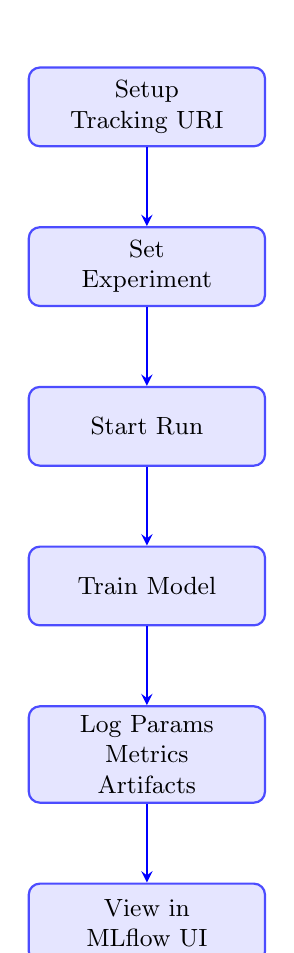
\begin{tikzpicture}[
    node distance=1cm,
    box/.style={rectangle, rounded corners, draw=blue!70, fill=blue!10, thick, minimum width=3cm, minimum height=1cm, align=center, font=\small},
    arrow/.style={->, >=stealth, thick, blue}
]

\node[box] (setup) {Setup\\Tracking URI};
\node[box, below=of setup] (experiment) {Set\\Experiment};
\node[box, below=of experiment] (run) {Start Run};
\node[box, below=of run] (train) {Train Model};
\node[box, below=of train] (log) {Log Params\\Metrics\\Artifacts};
\node[box, below=of log] (view) {View in\\MLflow UI};

\draw[arrow] (setup) -- (experiment);
\draw[arrow] (experiment) -- (run);
\draw[arrow] (run) -- (train);
\draw[arrow] (train) -- (log);
\draw[arrow] (log) -- (view);

\end{tikzpicture}
\end{center}

\subsection{Hyperparameter Tuning Workflow}

\vspace{0.5em}

\begin{center}
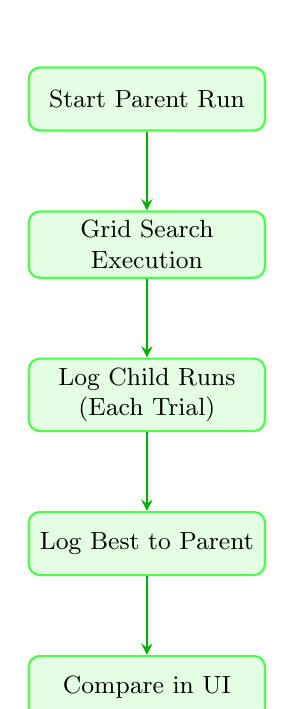
\begin{tikzpicture}[
    node distance=1cm,
    box/.style={rectangle, rounded corners, draw=green!70, fill=green!10, thick, minimum width=3cm, minimum height=0.8cm, align=center, font=\small},
    arrow/.style={->, >=stealth, thick, green!70!black}
]

\node[box] (parent) {Start Parent Run};
\node[box, below=of parent] (grid) {Grid Search\\Execution};
\node[box, below=of grid] (child) {Log Child Runs\\(Each Trial)};
\node[box, below=of child] (best) {Log Best to Parent};
\node[box, below=of best] (compare) {Compare in UI};

\draw[arrow] (parent) -- (grid);
\draw[arrow] (grid) -- (child);
\draw[arrow] (child) -- (best);
\draw[arrow] (best) -- (compare);

\end{tikzpicture}
\end{center}

\subsection{DVC + MLflow + Git Integration}

\vspace{0.5em}

\begin{center}
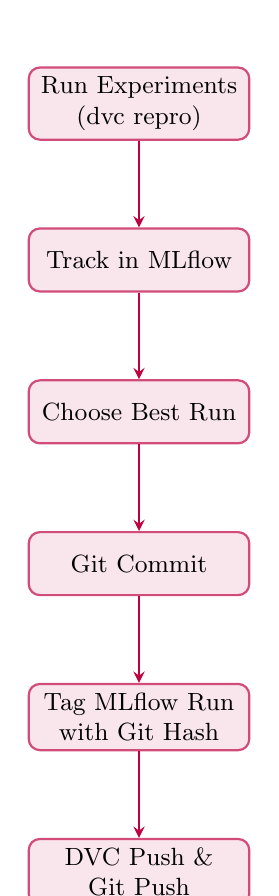
\begin{tikzpicture}[
    node distance=1.1cm,
    box/.style={rectangle, rounded corners, draw=purple!70, fill=purple!10, thick, minimum width=2.8cm, minimum height=0.8cm, align=center, font=\small},
    arrow/.style={->, >=stealth, thick, purple}
]

\node[box] (exp1) {Run Experiments\\(dvc repro)};
\node[box, below=of exp1] (mlflow) {Track in MLflow};
\node[box, below=of mlflow] (choose) {Choose Best Run};
\node[box, below=of choose] (commit) {Git Commit};
\node[box, below=of commit] (tag) {Tag MLflow Run\\with Git Hash};
\node[box, below=of tag] (push) {DVC Push \&\\Git Push};

\draw[arrow] (exp1) -- (mlflow);
\draw[arrow] (mlflow) -- (choose);
\draw[arrow] (choose) -- (commit);
\draw[arrow] (commit) -- (tag);
\draw[arrow] (tag) -- (push);

\end{tikzpicture}
\end{center}

\subsection{Model Registry Workflow}

\vspace{0.5em}

\begin{center}
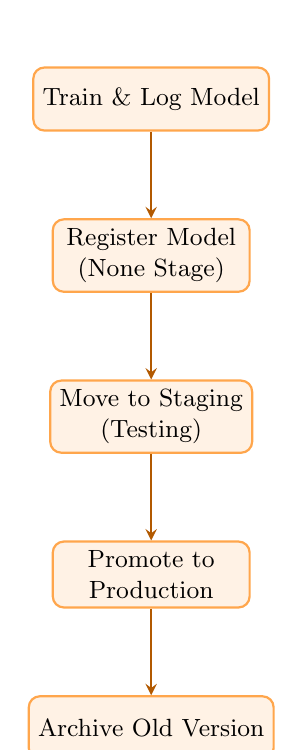
\begin{tikzpicture}[
    node distance=1.1cm,
    box/.style={rectangle, rounded corners, draw=orange!70, fill=orange!10, thick, minimum width=2.5cm, minimum height=0.8cm, align=center, font=\small},
    arrow/.style={->, >=stealth, thick, orange!70!black}
]

\node[box] (train) {Train \& Log Model};
\node[box, below=of train] (register) {Register Model\\(None Stage)};
\node[box, below=of register] (staging) {Move to Staging\\(Testing)};
\node[box, below=of staging] (prod) {Promote to\\Production};
\node[box, below=of prod] (archive) {Archive Old Version};

\draw[arrow] (train) -- (register);
\draw[arrow] (register) -- (staging);
\draw[arrow] (staging) -- (prod);
\draw[arrow] (prod) -- (archive);

\end{tikzpicture}
\end{center}

\newpage

% ========================
% SECTION 18: CONCLUSION
% ========================
\section{Conclusion and Key Takeaways}

\subsection{What You've Learned}

Throughout this comprehensive guide, you've mastered:

\begin{enumerate}[leftmargin=*]
    \item \textbf{MLflow Fundamentals}:
    \begin{itemize}
        \item Installation and setup
        \item Tracking URI configuration
        \item Experiment and run management
    \end{itemize}
    
    \item \textbf{Experiment Tracking}:
    \begin{itemize}
        \item Manual logging (parameters, metrics, artifacts)
        \item Autolog for automated tracking
        \item Nested runs for hyperparameter tuning
    \end{itemize}
    
    \item \textbf{Remote Collaboration}:
    \begin{itemize}
        \item Dagshub integration
        \item Team-wide experiment sharing
        \item Centralized tracking server
    \end{itemize}
    
    \item \textbf{DVC + MLflow + Git Integration}:
    \begin{itemize}
        \item Industry-standard workflow
        \item Runs vs commits distinction
        \item Proper rollback procedures
    \end{itemize}
    
    \item \textbf{Model Registry}:
    \begin{itemize}
        \item Model lifecycle management
        \item Stage transitions
        \item Compliance and auditability
    \end{itemize}
\end{enumerate}

\subsection{Core Principles to Remember}

\begin{infobox}{The Five Pillars of MLflow}
\begin{enumerate}[leftmargin=*]
    \item \textbf{Track Everything}: Parameters, metrics, artifacts, code
    \item \textbf{Organize Logically}: Experiments group related runs
    \item \textbf{Collaborate Effectively}: Use remote servers for team work
    \item \textbf{Commit Intentionally}: Runs are experiments, commits are decisions
    \item \textbf{Maintain Accountability}: Model registry for compliance
\end{enumerate}
\end{infobox}

\subsection{MLflow vs DVC: When to Use Each}

\begin{center}
\begin{tabular}{|p{0.45\textwidth}|p{0.45\textwidth}|}
\hline
\textbf{Use MLflow For} & \textbf{Use DVC For} \\
\hline
Experiment tracking and comparison & Data and model versioning \\
\hline
Model registry and lifecycle & Pipeline automation \\
\hline
Team collaboration on experiments & Reproducible workflows \\
\hline
Hyperparameter tuning tracking & Large file management \\
\hline
Model deployment decisions & Git-style data version control \\
\hline
\end{tabular}
\end{center}

\begin{notebox}
\textbf{Best Practice}: Use BOTH together!

\begin{itemize}[leftmargin=*]
    \item DVC for data/pipeline versioning
    \item MLflow for experiment tracking
    \item Git for code versioning
    \item Together: Complete MLOps solution
\end{itemize}
\end{notebox}

\subsection{The Complete MLOps Stack}

\begin{center}
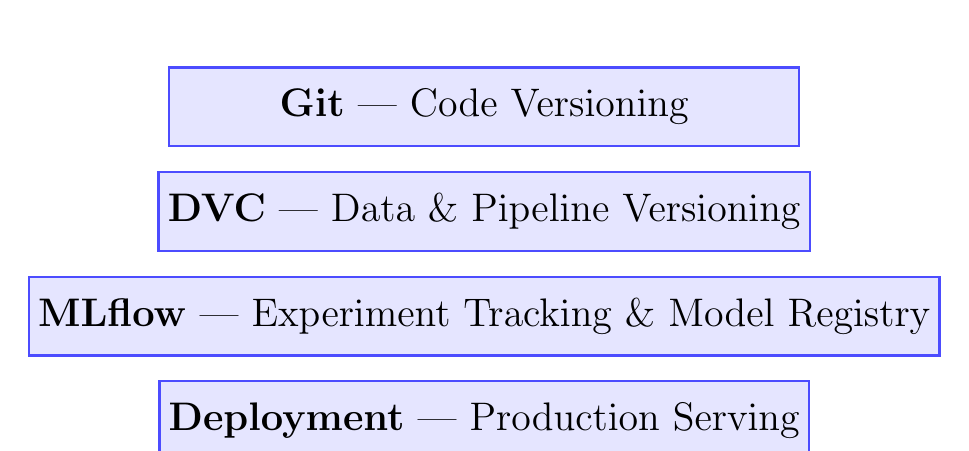
\begin{tikzpicture}[
    node distance=0.3cm,
    box/.style={rectangle, draw=blue!70, fill=blue!10, thick, minimum width=8cm, minimum height=1cm, align=center}
]

\node[box] (git) {\Large\textbf{Git} — Code Versioning};
\node[box, below=of git] (dvc) {\Large\textbf{DVC} — Data \& Pipeline Versioning};
\node[box, below=of dvc] (mlflow) {\Large\textbf{MLflow} — Experiment Tracking \& Model Registry};
\node[box, below=of mlflow] (deploy) {\Large\textbf{Deployment} — Production Serving};

\end{tikzpicture}
\end{center}

\subsection{Industry Workflow Recap}

\begin{examplebox}{The Complete Industry Process}
\begin{enumerate}[leftmargin=*]
    \item \textbf{Experiment Phase}:
    \begin{itemize}
        \item Run multiple experiments with MLflow tracking
        \item Compare results in MLflow UI
        \item Iterate on parameters and approaches
    \end{itemize}
    
    \item \textbf{Decision Phase}:
    \begin{itemize}
        \item Choose best run from MLflow
        \item Git commit the winning configuration
        \item Tag MLflow run with Git commit hash
    \end{itemize}
    
    \item \textbf{Deployment Phase}:
    \begin{itemize}
        \item Register model in MLflow Registry
        \item Move through stages: None → Staging → Production
        \item Monitor and maintain
    \end{itemize}
    
    \item \textbf{Maintenance Phase}:
    \begin{itemize}
        \item Archive old models (don't delete)
        \item Maintain audit trail
        \item Rollback using Git commit hash when needed
    \end{itemize}
\end{enumerate}
\end{examplebox}

\subsection{Critical Reminders}

\begin{warningbox}
\textbf{Never Forget}:

\begin{enumerate}[leftmargin=*]
    \item Always set tracking URI explicitly
    \item Runs are experiments, commits are decisions
    \item Archived $\neq$ Deleted (keep for compliance)
    \item Git commit hash is the rollback anchor
    \item MLflow tracks experiments, but Git + DVC enable rollback
    \item Team collaboration requires remote server (Dagshub/MLflow server)
    \item Log enough information to reproduce results
    \item Register production models in Model Registry
\end{enumerate}
\end{warningbox}

\subsection{Next Steps}

To continue your MLflow journey:

\begin{enumerate}[leftmargin=*]
    \item \textbf{Practice}: Set up MLflow in your own projects
    \item \textbf{Experiment}: Try different tracking configurations
    \item \textbf{Collaborate}: Set up Dagshub for team projects
    \item \textbf{Integrate}: Combine DVC + MLflow + Git workflow
    \item \textbf{Explore}: Advanced features like MLflow Projects, Model Serving
    \item \textbf{Contribute}: Join the MLflow community
\end{enumerate}

\subsection{Additional Resources}

\begin{itemize}[leftmargin=*]
    \item Official MLflow Documentation: \url{https://mlflow.org/docs/latest/index.html}
    \item MLflow GitHub Repository: \url{https://github.com/mlflow/mlflow}
    \item Dagshub Platform: \url{https://dagshub.com}
    \item MLflow Tutorials: \url{https://mlflow.org/docs/latest/tutorials-and-examples/index.html}
    \item DVC + MLflow Integration: \url{https://dvc.org/doc/use-cases/versioning-data-and-model-files}
\end{itemize}

\subsection{Final Thoughts}

MLflow has become an essential tool in the modern ML engineer's toolkit. By providing:

\begin{itemize}[leftmargin=*]
    \item \textbf{Experiment tracking} that scales from solo projects to large teams
    \item \textbf{Model registry} that ensures governance and compliance
    \item \textbf{Integration capabilities} that work with existing tools
    \item \textbf{Flexibility} to adapt to various workflows
\end{itemize}

MLflow enables you to move from experimental notebooks to production-ready ML systems with confidence.

\begin{infobox}{The Golden Rule of MLOps}
\textbf{Track everything, commit intentionally, deploy confidently.}

\vspace{0.5em}

With MLflow, DVC, and Git working together, you have complete control over your ML lifecycle — from the first experiment to the last model retirement.
\end{infobox}

\vspace{2em}
\hrule
\vspace{0.5em}
\begin{center}
\textit{End of MLflow Complete Guide}

\vspace{1em}

\textit{"Without data, you're just another person with an opinion."}\\
\textit{— W. Edwards Deming}

\vspace{1em}

\textit{With MLflow, your data becomes actionable insights!}
\end{center}

\end{document}